% Revisions to the Kepler Conjecture.
% Author: Hales, Harrison, McLaughlin, Nipkow, Obua, Zumkeller

% email: hales@pitt.edu
%
% latex format

% History:
% Branched from dcg_errata.tex on Oct 8, 2008
% Common material deleted from dcg_errata.tex on Nov 2, 2008.

%% ISSUES:
% XX
% Accents on VN names.

% Global changes:
% voice: Hales did this -> The original proof does this.


\documentclass[11pt]{amsart}
%\documentclass{llncs}
\usepackage{graphicx}
\usepackage{url}
\usepackage{amsfonts}
\usepackage{amscd}
\usepackage{amssymb}
\usepackage{alltt}
%\usepackage{amsmath,amsthm}

% automatically generate revision number by
% svn propset svn:keywords "LastChangedRevision" revision.tex
\def\svninfo{{\tt
  filename: revision.tex\hfill\break
  PDF generated from LaTeX sources on \today; \hfill\break
  Repository Root: https://flyspeck.googlecode.com/svn \hfill\break
  SVN $LastChangedRevision$
  }
  }
%-%


% Math notation.
\def\op#1{{\text{#1}}}
\newcommand{\mc}[1]{{\mathcal{#1}}}
\newcommand{\ring}[1]{\mathbb{#1}}
%\def\to{{\ensuremath{\quad\Longrightarrow\quad}}}
\def\lto{\ensuremath{\,\leadsto\,}}
\def\dih{\op{dih}}
\def\line{$\ell$}
\def\text{\hbox}
\def\sz{small} % was scriptsize
\def\|{{\hskip0.1em|\hskip-0.15em|\hskip0.1em}}

% Typesetting:
\def\coloneq{\mathrel{\mathop:}=}
\def\sfrac#1#2{{\textstyle \frac {#1} {#2}}}
\def\eqref#1{(\ref{#1})}
\def\rmx{\rm}


% Flyspeck:
\def\pt{\mathrm{pt}}
\def\doct{\delta_{\mathrm{oct}}}
\def\asolid{\mathrm{a}}
\def\sqroot{\mathrm{sqrt}}
\def\rcp{\mathrm{rcp}}
\def\bstein{\mathrm{B}}

% Harrison's macros:
\newcommand{\nat}{\mbox{$\protect\mathbb N$}}
\newcommand{\num}{\mbox{$\protect\mathbb Z$}}
\newcommand{\rat}{\mbox{$\protect\mathbb Q$}}
\newcommand{\real}{\mbox{$\protect\mathbb R$}}
\newcommand{\complex}{\mbox{$\protect\mathbb C$}}
\newcommand{\xxx}{\mbox{$\protect\mathbb X$}}
\newcommand{\bool}{\mbox{$\protect\mathbb B$}}

\newcommand{\lamb}[1]{\lambda #1.\:}
\newcommand{\eps}[1]{\varepsilon #1.\:}
\newcommand{\all}[1]{\forall #1.\:}
\newcommand{\ex}[1]{\exists #1.\:}
\newcommand{\exu}[1]{\exists! #1.\:}

\newcommand{\True}{\top}
\newcommand{\False}{\bot}
\newcommand{\Not}{\neg}
% \newcommand{\And}{\wedge}
\let\And=\wedge                    % Another definition in amsmath

\newcommand{\Or}{\vee}
\newcommand{\Imp}{\Rightarrow}
\newcommand{\Iff}{\Leftrightarrow}

\newcommand{\entails}{\vdash}
\newcommand{\sequent}{\to}
\newcommand{\proves}{\vdash}

\newcommand{\Ands}{\bigwedge}
\newcommand{\Ors}{\bigvee}

\newcommand{\BQ}{\mbox{$\ulcorner$}}
\newcommand{\BEQ}{\mbox{\raise4pt\hbox{$\ulcorner$}}}
\newcommand{\EQ}{\mbox{$\urcorner$}}
\newcommand{\EEQ}{\mbox{\raise4pt\hbox{$\urcorner$}}}

\let\psubset=\subset                    % Pure TeX: thanks to MAJ %
\let\subset=\subseteq
\let\psupset=\supset
\let\supset=\supseteq

\newcommand{\powerset}{\wp}             % This is pretty dire...  %

\newcommand{\Union}{\cup}
\newcommand{\Inter}{\cap}
\newcommand{\Unions}{\bigcup}
\newcommand{\Inters}{\bigcap}

%\newcommand{\binom}[2]{{{#1} \choose {#2}}}

%\newcommand{\proof}{{\bf \noindent Proof:\ }}
%\newcommand{\qed}{Q.E.D.}

\newcommand{\Rule}{\infer}

\newcommand{\restrict}{\upharpoonright} % This is lousy and must be fixed! %

\newcommand{\bigsqcap}{\mbox{\Large{$\sqcap$}}}

\newcommand\leb{\lbrack\!\lbrack}
\newcommand\reb{\rbrack\!\rbrack}
\newcommand{\sem}[1]{\leb #1 \reb}

\newcommand{\BA}{\begin{array}[t]{l}}
\newcommand{\EA}{\end{array}}

\newcommand{\sqle}{\sqsubseteq}
\newcommand{\sqlt}{\sqsubset}

\newcommand{\from}{\leftarrow}
\newcommand{\too}{\twoheadrightarrow}

\newcommand{\Los}{{\L}o{\'s}}
\newcommand{\del}{\partial}

\newcommand{\QUOTE}[1]{\mbox{$\BQ #1 \EQ$}}
\newcommand{\floor}[1]{\mbox{$\left\lfloor #1 \right\rfloor$}}
\newcommand{\ceil}[1]{\mbox{$\left\lceil #1 \right\rceil$}}
\newcommand{\bracket}[1]{\mbox{$\left\langle #1 \right\rangle$}}

\newcommand{\until}{\;\mbox{\tt U}\;}

\newcommand{\tm}{$^{\mbox{{\tiny TM}}}$}
\newcommand{\registeredtrademark}{\Pisymbol{psy}{210}}

\newcommand{\itanium}{Intel{\registeredtrademark} Itanium{\registeredtrademark}}
\newcommand{\pentium}{Intel{\registeredtrademark} Pentium{\registeredtrademark}}

% This is an infix modulus operator

%\newcommand{\mod}{\mbox{\tt{ mod }}}

% This (\imod) is for congruences mod.

\makeatletter
\def\imod#1{\allowbreak\mkern10mu({\operator@font mod}\,\,#1)}
\makeatother

% This is stuff for boxes, stolen from HOL documentation

\newcommand\HOLSpacing{12pt}

\newlength{\hsbw}
\setlength{\hsbw}{\textwidth}
\addtolength{\hsbw}{-\arrayrulewidth}
\addtolength{\hsbw}{-\tabcolsep}

%\newenvironment{boxed}{\begin{flushleft}
% \begin{tabular}{@{}|c@{}|@{}}\hline
% \begin{minipage}[b]{\hsbw}
% \vspace*{.06in}
% \begingroup\small\baselineskip\HOLSpacing}{\endgroup\end{minipage}\\ \%hline
% \end{tabular}
% \end{flushleft}}

% Some additional "log-like" functions

\newcommand{\asn}{\mathop{\mathrm{asn}}\nolimits}
\newcommand{\acs}{\mathop{\mathrm{acs}}\nolimits}
\newcommand{\atn}{\mathop{\mathrm{atn}}\nolimits}
\newcommand{\atan}{\mathop{\mathrm{atan}}\nolimits}
\newcommand{\asin}{\mathop{\mathrm{asin}}\nolimits}
\newcommand{\acos}{\mathop{\mathrm{acos}}\nolimits}

% Handy for multivariate stuff

\newcommand{\xs}{\overline{x}}

% Hyphenation stuff

\hyphenation{dijk-stra}

\newcommand{\citeN}{\cite}



\newtheorem{definition}[section]{Definition}
\newtheorem{thm}{Theorem}
\newtheorem{lemma}{Lemma}
\newtheorem{assumption}[section]{Assumption}
\newtheorem{corollary}[section]{Corollary}
\newtheorem{remark}[section]{Remark}


\parindent=0pt
\parskip=\baselineskip

%%%%%%%%%%%%%%%%%%%%%%%%%%%%%%%%%%

\begin{document}

\title{A revision of the proof of the Kepler Conjecture}

\author[Hales]{Thomas C. Hales}
\address[T.~Hales]{Math Department, University of Pittsburgh}
\email{hales@pitt.edu}

\author[Harrison]{John Harrison}
\address[J.~Harrison]{Intel Corporation,  JF1-13, 2111 NE 25th Avenue
 Hillsboro, OR 97124
 USA}
\email{johnh@ichips.intel.com}

\author[McLaughlin]{Sean McLaughlin}
\address[S.~McLaughlin]{Carnegie Mellon University}

\author[Nipkow]{Tobias Nipkow}
\address[T.~Nipkow]{Department for Informatics, Technische Universit\"at
M\"unchen}
\email{\url{www.in.tum.de/~nipkow}}

\author[Obua]{Steven Obua}
\address[S.~Obua]{Department for Informatics, Technische Universit\"at
M\"unchen}

\author[Zumkeller]{Roland Zumkeller}
\address[R.~Zumkeller]{\'Ecole Polytechnique, Paris}

\begin{abstract}
The Kepler conjecture asserts that no packing of congruent balls in three-dimensional Euclidean space 
has density greater than that of the face-centered cubic packing.  The original proof,
announced in 1998 and published in 2006, is long and complex. The process of  revision and review did not end with the publication of the proof.
This article summarizes the current status of several long-term iniatiatives to
reorganize the original proof into a more transparent form and to provide a greater
level of certification of the correctness of the computer code and other details of the proof.
A final section contains an errata to the original proof of the Kepler conjecture.
\end{abstract}


\maketitle

\section{Introduction}

In 2006, {\it Discrete and Computational Geometry} devoted an issue to the
proof of the Kepler Conjecture on sphere packings, which asserts that no
packing of congruent balls in three-dimensional Euclidean space can
have density greater than that of the face-centered cubic packing \cite{Hales:2006:DCG}.
This density is $\pi/\sqrt{18}$.

The proof is long and complex.  The editors' forward to that issue remarks
that ``the reviewing of these papers ws a particularly enormous and daunting task.''
``The main portion of the reviewing took place in a seminar run at E\"otvos University
over a 3 year period.  Some computer experiments were done in a detailed check.
The nature of this proof, consisting in part of a large number of inequalities having
little internal structure, and a complicated proof tree, makes it hard for humans
to check every step reliably.  Detailed checking of specific assertions found them to
be essentially correct in every case tested.  The reviewing process produced in the
reviewers a strong degree of conviction of the essential correctness of the proof
approach, and that the reduction method led to nonlinear programming problems of
tractable size.''

The process of review and revision did not end when the proof was published.
This article summarizes the current status of several long-term iniatiatives to
reorganize the original proof into a more transparent form and to provide a greater
level of certification of the correctness of the computer code and other details of the proof.

In this article, the {\it original proof} refers to the proof published
in \cite{Hales:2006:DCG}.

\section{The Flyspeck project}

\subsection*{Formal proof}

A formal proof is a proof in which every logical inference has been checked, all the way back to the foundational axioms of mathematics.  No step is skipped no matter how obvious it may be to a mathematician.  
A formal proof may be less intuititve, and yet is less susceptible to logical
errors.  Because of the large number of inferences involved, a computer is generally used to check the steps of a formal proof.

It is generally a large labor-intensive
undertaking to transform a traditional proof
into a formal proof.   The first stage is generally to expand the traditional proof in greater detail.  This stage fills in steps that a mathematician would regard as obvious,  works out arguments that the original proof leaves to the reader,  and supplies the assumed background knowledge.  
In a final stage, the detailed text is transcribed into a computer-readable format inside
a computer proof assistant.  The proof assistant  contains  mathematical axioms, logical rules of inference, and a collection of previously proved theorems. 
It validates each new lemma by stepping through each inference.  No other currently available technology is able to provide levels of certification of a complex mathematical proof that is remotely comparable to that available by formal computer verification.  A general overview
of formal proofs can be found at~\cite{gonthier:2008:formal}, \cite{Hales:2008:formal}, \cite{Harrison:2008:formal}.

Proof assistants differ in detail in the way they treat the formalization
of  a theorem that is itself a computer verification (such as
the proof of the four color theorem or the proof of the Kepler conjecture).
In general, a formal proof of a computer verification can be viewed
as a formal proof of the correctness of the computer code used in the
verification.  That is, the formal proof certifies that the the code
is a bug-free implementation of its specification.





\subsection*{Formal proof of the Kepler conjecture}

The purpose of the Flyspeck project is to give a formal proof of the Kepler conjecture.  (The project name {\it Flyspeck} comes from the acronym {\it FPK}, for the {\it Formal} {\it Proof} of the {\it Kepler} conjecture.)  This is the most complex formal proof ever undertaken.  We estimate that it may take about twenty work-years to complete this formalization project.  

The Flyspeck project is introduced in the article~\cite{hales:DSP:2006:432}.
The project page gives the latest project developments~\cite{website:FlyspeckProject}.
The project is now at an advanced stage of development; in fact, we estimate that the project is now about half-way complete.  
One of the main purposes of this article is to present a summary of the current status of this project.

In the original proof of the Kepler conjecture, there were three major pieces of computer code and a long mathematical text.
There have have been three Ph.D. theses on the Flyspeck
project, one devoted to each of the three major pieces of computer code.
The first piece of computer code enumerates all tame graphs.
(The definition of tameness is rather intricate; its key property is that the set of tame graphs 
includes all graphs that give a potential counterexample to the conjecture.)
G. Bauer's thesis, together with subsequent 
work with T. Nipkow, completes the formal
proof of the enumeration of tame graphs~\cite{NipkowBS-IJCAR06}.
Section~\ref{sec:graph} gives a summary of this formalization project.
The second piece of computer code generates and runs some $10^5$ linear
programs.   These linear programs show that none of the potential counterexamples
to the Kepler are actual counterexamples.  S. Obua's thesis develops the
technology to generate and verify the linear programs inside the proof assistant Isabelle~\cite{obua:phd}. 
Section~\ref{sec:lp} describes this research.
The final piece of computer code uses interval arithmetic to verify nonlinear inequalities.  R. Zumkeller's thesis develops nonlinear inequality proving inside the proof assistant Coq~\cite{roland-thesis}.  Section~\ref{sec:zumkeller} gives an example of this work.  In the years following the publication of the original proof, S. McLaughlin has  reworked and largely rewritten the entire body of code in a form that is more transparent and more amenable to formalization.  Section~\ref{sec:code} points out some difficulties
in verifying the computer code in its original form and
documents the reimplementation.

The written part of the proof has also been substantially revised with aims of the Flyspeck project in mind.   Section~\ref{sec:blueprint} compares this revised text with the original.  There is now a good match between the mathematical background assumed in the text and the mathematical material that is available in the proof assistant HOL Light.  Section~\ref{sec:ordinary} describes the current level of support in HOL Light for the formalization of Euclidean space and measure theory.

The ultimate aim is to develop a complete formal proof of the Kepler
conjecture within a single proof assistant.  Because of the scope of 
the problem and the number of researchers involved, different proof
assistants have been used for different parts of the proof:
Isabelle/HOL for graph enumeration and linear programming, Coq for
nonlinear inequality verification, and HOL Light for background
in Euclidean geometry and the text.  This raises the issue of how
to translate a formal proof automatically from one proof assistant to another.
Implementations of automated translation among the
proof assistants HOL, Isabelle, and Coq can be found 
at~\cite{obua:import}, \cite{McLaughlin:2006:IJCAR}, \cite{wiedijk:encoding},
\cite{695027}.



\section{Blueprint edition of the Kepler conjecture}
\label{sec:blueprint}

The starting point of a formal proof is a standard mathematical proof in which every step
has been expanded in great detail.  The original proof of the Kepler conjecture was not written
in a manner to permit easy formalization.  A formalization-friendly version of the proof has
now been prepared, which we refer to as the blueprint edition~\cite{hales:2008:blueprint}, \cite{hales:2008:collection}.  It contains far more detail than the original proof.  This section 
compares this expanded text with the original.\footnote{The formalization of the blueprint text started in
2008 with work of J. Rute (CMU) and the Hanoi Flyspeck group. The members of this group are Tran Nam Trung, Nguyen Tat Thang, Hoang Le Truong, Nguyen Quang Truoung, Vu Khac Ky, Nguyen Anh Tam, Nguyen Tuyen Hoang, Nguyen Duc Phuong, Vuong Anh Quyen, Phan Hoang Chon, and managed by Ta Thi Hoai An.  This is still at an early stage; completion is still years away.}

\subsection*{Collection in elementary geometry}

The original proof of the Kepler conjecture contains a large number of lemmas that can be
expressed in the first-order language of the real numbers; that is, they can be expressed in
the syntax of first-order logic with equality (allowing quantifiers $\forall x$, $\exists x$ with variables
running over the real numbers), the real constants $0$, $1$, and ring operations $(+)$, $(-)$,
$(\cdot)$ on $\ring{R}$.  In fact, L. Fejes T\'oth's formulation of the Kepler conjecture to
a problem in a finite number of variables can itself be expressed in the
first-order language of the real numbers.  (For this, the truncation used by L. Fejes T\'oth must be modified slightly so that the truncated Voronoi cells are polyhedra.)  Thus, it should come as no surprise that many
of the intermediate lemmas in the proof can also be expressed in this manner.

For example, consider the statement asserting the existence of a circumcenter of a triangle: 
if three points in the plane are not collinear, then there exists a
point in the plane that is equidistant from all three.  This can be expressed in elementary terms
as follows:  for every $(x_1,y_1)$, $(x_2,y_2)$, $(x_3,y_3)$, if there do not exist $t_1,t_2,t_3$
for which $t_1 (x_1,y_1) + t_2 (x_2,y_2)+ t_3 (x_3,y_3) = (0,0)$ and $t_1+t_2+t_3=1$, then there exists
$(x,y)$ such that 
$$
  (x-x_1)^2 + (y-y_1)^2 = (x-x_2)^2 + (y-y_2)^2 = (x-x_3)^2 + (y-y_3)^2. 
$$



A collection of about 200 lemmas that can be expressed in elementary terms has been extracted from 
the original proof and placed in a separate collection~\cite{hales:2008:collection}.  This has
several advantages.  First of all, these lemmas, although elementary, are precisely the parts of the
original proof that put the greatest burden on the reader's geometrical imagination.  (Many of these
lemmas deal with the existence or non-existence of configurations of several points in $\ring{R}^3$ subject to
various metric constraints.)  Also, the lemmas can be stated without reference to the Kepler conjecture and all of the
technical notions that have been introduced to give a proof.
Finally, the proofs rely on similar methods and are best considered
together~\cite{1271687}.  Section~\ref{sec:ordinary} on {\it Enchanced Automation} gives an approach to proving the lemmas in this collection.

 

\subsection*{Background material}

All of the necessary background material for the proof has been supplied.  As we mentioned above, there is now a close
match between what the blueprint edition assumes as background and what the proof assistant {\it HOL Light}
provides, as described in Section~\ref{sec:ordinary}.  The blueprint edition develops 
substantial background
material in trigonometry, measure and integration, hypermaps, and fans.   It turns out
that only a small number of {\it primitive} volumes need to be computed for the proof of the Kepler
conjecture. These primitives include the volume of a ball, a tetrahedron, and right circular cone.  
No line or surface integrals are required.

A hypermap is a finite set $D$ with three permutations $e,n,f$ that compose to the identity $e\circ n\circ f= I$.  A hypermap is the
combinatorial structure used by Gonthier in his formal proof of the four color theorem.  In 2005,
the proof of the Kepler conjecture was rewritten in terms of hypermaps, because it is better suited
for formal proofs than planar graphs.  Roughly speaking, a fan is a geometric realization of a hypermap,
adapted to needs of sphere packings in three dimensions.

The Jordan Curve theorem has been formalized as a step in the Flyspeck project~\cite{Hales:2007:jordan}.  In fact, something weaker than the Jordan curve theorem
is needed for the Flyspeck project.  The only simple closed curves that arise are curves on
the surface of a unit sphere consisting of a finite number of arcs of great circles.  That is,
only a (spherical) polygonal version of the Jordan curve theorem is needed.  The Jordan curve
theorem is used to compute the Euler characteristic of the hypermap formed by a fan.  Planarity of a hypermap is defined by a condition on its Euler characteristic.  The result is a proof that a cluster of spheres determine a fan, which in turn determines a planar hypermap.
The background chapter on fans in the blueprint edition contains detailed proofs of these facts.


The blueprint edition also contains several introductory essays that give a gentle introduction
to the main concepts in the proof, including the computational methods embedded in computer code.




\section{Formalizing the ordinary mathematics}
\label{sec:ordinary}

The computer code in Flyspeck has so far received the lion's share of the
formal effort. This is entirely reasonable since there are, or at least were,
real questions about the feasibility of reproducing these results in a formal
way. However, the Flyspeck proof includes a large amount of `ordinary'
mathematics, which also needs to be formalized. Here we are on fairly safe
ground in principle, because by now we understand the formalization of
mainstream mathematics quite well~\cite{wiedijk-17}. It is safe to predict that
this formalization can be done, and we can even hope for a reasonably accurate
estimate of the effort involved. Nevertheless, the formalization is certainly
non-trivial and will require considerable work. Here we describe some of the
work on formalizing Euclidean space and measure theory, and the development of
further proof automation, which should be useful in this endeavor.

\subsection*{Formalizing Euclidean space}

Much of our work has been devoted to developing a solid general theory of
Euclidean space $\real^N$ \cite{harrison-euclidean}. For Flyspeck, we
invariably just need the special case $\real^3$. While some concepts, e.g.
vector cross products, are specific to $\real^3$, most of the theory has been
developed for general $\real^N$ so as to be more widely applicable. The theorem
prover HOL Light \cite{harrison-demo} is based on a logic without dependent
types, but we can still encode the index $N$ as a type (roughly, an arbitrary
indexing type of size $N$). This means that theorems about specific sizes like
$3$ really are just type instantiations of theorems for general $N$ stated with
polymorphic type variables. The theory contains the following:

\begin{itemize}

\item Basic properties of vectors in $\real^N$, linear operators and matrices,
dimensions of vector subspaces and other bits of linear algebra. For example,
the following is a formal statement of the theorem that a square matrix $A'$ is
a left inverse to another one $A$ iff it is a right inverse. Note that the
double use of the same type variable $N$ constrains the theorem to square
matrices:

\begin{\sz}
\begin{alltt}
|- \(\forall\)A:real^N^N A':real^N^N. (A ** A' = mat 1) \(\Iff\) (A' ** A = mat 1)
\end{alltt}
\end{\sz}

\item Metric and topological notions like distances, open sets, closure,
compactness and paths. Some of these are very general, others are more specific
to Euclidean space. Some results include the Heine-Borel theorem, the Banach
fixed-point theorem and Brouwer's fixed-point theorem. The following is a
formal statement that continuous functions preserve connectedness.

\begin{\sz}
\begin{alltt}
|-  \(\forall\)f:real^M->real^N s. f continuous_on s \(\And\) connected s \(\Imp\) connected(IMAGE f s)
\end{alltt}
\end{\sz}

\item Properties of convex sets, convex hulls, cones etc. Results include
Helly's theorem, Carath\'eodory's theorem, and various classic results about
separating and supporting hyperplanes. The following states a simpler but not
entirely trivial result that convex hulls preserve compactness.

\begin{\sz}\begin{alltt}
|- \(\forall\)s:real^N->bool. compact s \(\Imp\) compact(convex hull s)
\end{alltt}\end{\sz}

\item Sequences and series of vectors and uniform convergence, Fr\'echet
derivatives and their properties, up to various forms of the inverse function
theorem, as well as specific 1-dimensional theorems like Rolle's theorem and
the Mean Value Theorem. Here is the formal statement of the chain rule for
Fr\'echet derivatives.

\begin{\sz}\begin{alltt}
|- \(\forall\)f:real^M->real^N g:real^N->real^P f' g'.
        (f has_derivative f') (at x) \(\And\)
        (g has_derivative g') (at (f x))
        \(\Imp\) ((g o f) has_derivative (g' o f')) (at x)
\end{alltt}\end{\sz}

\end{itemize}

\subsection*{Formalizing measure theory}

Although the basic Euclidean theory is an important foundation, and many of the
concepts like `convex hull' are used extensively in the Flyspeck mathematics,
perhaps the most important thing to formalize is the concept of volume.

We define integrals of general vector-valued functions over subsets of
$\real^N$, using the Kurzweil-Henstock gauge integral definition. We develop
all the usual properties such as additivity and the key monotone and dominated
convergence theorems. We also develop a theory of {\em absolutely} integrable
functions, where both $f$ and $|f|$ are gauge integrable; this is known to
coincide with the Lebesgue integral. Here is a formal statement of the simple
theorem that integration preserves linear scaling:

\begin{\sz}
\begin{alltt}
|- \(\forall\)f:real^M->real^N y s h:real^N->real^P.
        (f has_integral y) s \(\And\) linear h \(\Imp\) ((h o f) has_integral h(y)) s
\end{alltt}
\end{\sz}

Using this integral applied to characteristic functions, we develop a theory of
(Lebesgue) measure, which of course gives volume in the 3-dimensional case. The
specific notion `measure zero' is formalized as {\tt negligible}, and we also
have a general notion of a set having a finite measure, and a function {\tt
measure} to return that measure when it exists. For example, this is the basic
additivity theorem:

\begin{\sz}
\begin{alltt}
|- \(\forall\)s t. measurable s \(\And\) measurable t \(\And\) DISJOINT s t
         \(\Imp\) measure(s UNION t) = measure s + measure t
\end{alltt}
\end{\sz}

We have proved that various `well-behaved' sets such as bounded convex ones and
compact ones, or more generally those with negligible frontier (boundary) are
measurable, e.g.

\begin{\sz}
\begin{alltt}
|- \(\forall\)s:real^N->bool. bounded s \(\And\) negligible(frontier s) \(\Imp\) measurable s
\end{alltt}
\end{\sz}

The main lack at the moment is a set of results for actually computing the
measures of specific sets, as needed for Flyspeck. We can evaluate most basic
1-dimensional integrals by appealing to the Fundamental Theorem of Calculus,
but we need to enhance the theory of integration with stronger Fubini-type
results so that we can evaluate multiple integrals by iterated one-dimensional
integrals. This work is in progress at the time of writing.

\subsection*{Enhanced automation}

Using coordinates, many non-trivial geometric statements in $\real^3$, or other
Euclidean spaces of specific finite dimension, can be reduced purely to the
elementary theory of reals. This is known to be decidable using quantifier
elimination \cite{tarski-decision,collins,hormander-pdo2}. However, in practice
this is often problematic because quantifier elimination for nonlinear formulas
is inefficient. The problem is particularly severe if we want to have any kind
of {\em formal} proof, as we do in Flyspeck, since producing such a proof
induces further slowdowns \cite{mahboubi-hormander,mclaughlin-harrison}. With
this in mind, we have explored a different approach to the case of purely
universally quantified formulas \cite{harrison-sos}, based on ideas of Parrilo
\cite{parrilo-semidefinite}. This involves reducing the initial problem to
semidefinite programming, solving the SDP problem using an external tool and
reconstructing a `sum-of-squares' (SOS) certificate that can easily be formally
checked.

For example, suppose we wish to verify that if a quadratic equation $a x^2 + b
x + c = 0$ has a real root, then $b^2 \geq 4 a c$. Using the SDP solver we find
an algebraic certificate $b^2 - 4 a c = (2 a x + b)^2 - 4 a (a x^2 + b x + c)$,
from which the required fact follows easily: $(2 a x + b)^2 \geq 0$ because it
is a square, and $4 a (a x^2 + b x + c) = 0$ because $x$ is a root, and so we
deduce $b^2 - 4 a c \geq 0$. This method seems very useful for automating
routine nonlinear reasoning in a way that is easy and quick to formally verify,
so that we don't have to rely on the correctness of a complicated program. It
is even capable of solving the coordinate forms of some of the simpler Flyspeck
inequalities directly, though it seems unlikely to be competitive with
customized nonlinear optimization methods as implemented by Zumkeller. For
example, one simple Flyspeck inequality is the following, which after being
reduced to a real problem with 9 variables (three coordinates for each point)
is solved by SOS in a second:
$$ \|u - v\| \geq 2 \And \|u - w\| \geq 2 \And \|v - w\| \geq 2 \And
   \|u - v\| < \sqrt{8}
   \Imp \|w - (u + v)/2\| > \|u - v\|/2
$$

A quite different approach to geometric theorem proving is to work in the
setting of a general real vector space or normed real vector space. In this
case, other decision methods are available \cite{solovay-jointpaper}. In
particular, one of these decision procedures that we have implemented in HOL
Light can sometimes handle simple forms of spatial reasoning in a purely
`linear' way, and so be much more efficient than the direct reduction to
coordinates, even if we do in fact have a specific dimension in mind. One
real example from formalizing complex analysis is the following in $\real^2$:
$$ |\|w - z\| - r| = d \And \|u - w\| < d/2 \And \|x - z\| = r
   \Imp d/2 \leq \|x - u\|
$$




\section{Standard ML reimplementation of code}
\label{sec:code}

\subsection*{Code}




The original proof of the Kepler
Conjecture relies significantly
on computation. Computer code is used extensively, and is
central both to the correctness of the result and to a thorough
understanding of the proof. 

  There are four major difficulties with understanding and verifying
the original code base. The first and most glaring difficulty is
simply the amount of code. At the website~\cite{website:Hales:1998:Code}
that posts the code for the original proof,
there are well over 50,000 lines of programs in Java, C++, and
Mathematica. This represents only the calculations that Hales did himself.
Samuel Ferguson also completed many of the calculations with a completely
different code base of 137,000\footnote{There is a large amount of
code copying in Ferguson's code, resulting in a much larger code base.
The number of distinct lines is difficult to measure} lines of C. By
contrast, the proof of the Four Color Theorem by Robinson \textit{et.
al.}~\cite{Robertson:1997:JCTB} is less than 3,000 lines of C.

Another difficulty is in the organization of the code. The
calculations were done over the space of four years and involved % 10->4, tch, Oct 11, 2008
thousands of executions of the various programs. The variety of
computational tasks include, among others, estimating global bounds on
inequalities using nonlinear methods, proving inequalities rigorously
using interval arithmetic, generating graphs satisfying certain
properties, generating linear programs from graphs, and bounding
linear programs. Despite a labeling scheme used in the original proof 
to uniquely
identify his calculations, some computations relied upon by the proof
are difficult to find in the original source code. 
Ferguson has no such labeling scheme.  To locate, for
instance, computation ``CALC-821707685'' from the original proof~\cite[p.159]{Hales:2006:DCG}, one can search on the website~\cite{website:Hales:1998:Code} in
vain.  While records
of the computations were made, it is not always an easy matter
to find them without further guidance.

The third difficulty lies in the complexity of the implementation. For instance,
the software  developed to prove the inequalities upon which the original
proof rests is relatively complicated. Processing power at the time
(1994-1998) was just barely capable of completing the computations he
requested. To keep the length of execution to days or weeks instead of
months or years, the code is extensively optimized. The
optimizations were often implemented without comment in the source,
and in some cases are difficult to understand.  

Finally, Hales uses C++ and Ferguson uses C to carry out
\emph{interval arithmetic} calculations. In the process, they
explicitly set the IEEE 754~\cite{IEEE:1985:IEE754} rounding modes on
the floating point unit. There are a number of difficulties with using
floating point numbers and rounding modes directly. The first is that
reasoning about floating point instructions requires a relatively deep
understanding of the machine architecture~\cite{Monniaux:2008:TOPLAS}.
For instance, setting the rounding mode\footnote{In the C++ code
base the rounding modes are explicitly changed at least 400 times.}
changes the state of the processor itself. Such an instruction has a
global effect on all subsequent floating point computations. Moreover,
compilers, libraries, and even processors are notorious for unsound
implementations of the 754 standard. A GCC mailing list entry from
1998\footnote{\url{http://gcc.gnu.org/ml/gcc/1998-02/msg00998.html}},
the year the Kepler project was completed, contains the following
comment (after describing fixes for a number of other 754-related
bugs): ``When you use fpu/cpu to do rounding, you have to mark the
variable volatile. Otherwise, the compiler may do something  you don't
want.'' On the other hand, the volatile keyword is not well defined by
%% XX well defined or not defined at all.
the C language definition~\cite{Kernighan:1988:C}, meaning that a C
program using the volatile keyword is undefined by the
language definition. This is an unsatisfactory state of affairs.

% ------------------------------------------------------------------------------
%  Motivation                                                                   
% ------------------------------------------------------------------------------



\subsection*{Motivation and current status}
\label{sec:sean}

Our motivation in this work has been to bring the computational aspects of
the Kepler conjecture closer to the level of simplicity and clarity
necessary for formalization by a proof assistant. Our goals are:

\begin{enumerate}
\item The code should be rewritten in a functional language with a
  rigorous definition whose semantics resembles those supported by
  proof assistants such as HOL Light and Coq.
\item The implementation should be written in a subset of the language
  that is easily translatable to the object languages of Coq and HOL
  Light. This means it should not, for instance, use features such as state
  (references) that do not have obvious analogues in proof assistants.
\item The implementation should  avoid the use of floating
  point numbers and rounding modes.
\item The code should be organized in such a way that any
  computation upon which the proof relies can be evaluated from a single
  interface.  This will allow Flyspeck developers to easily find and
  check the paper results during the formalization process.
\end{enumerate} 

\noindent This
work is in the spirit of Robinson, \textit{et.
al.}~\cite{Robertson:1997:JCTB}, which simplified the original code of
Appel and Haken~\cite{Appel:1986:FourColor}, and was used by Gonthier to
construct the fully formal proof~\cite{gonthier:2008:formal} in the
Coq proof assistant. 

We chose Standard ML for the reimplementation for a number of reasons.
It has a formal definition~\cite{Milner:1990:SML}, and thus programs
have a meaning apart from the particular compiler used. It has a
foreign function interface that allows us to use external libraries
with relative ease. It has an expressive module system, and thus it is
possible to write the code with respect to an abstract libraries and
arithmetics. This allows us, for instance, to use multiple independent
implementations of interval arithmetic such as
MPFI~\cite{Revol:2005:MPFI}, as well as our own implementation using
floating point numbers. SML also has a very efficient
compiler~\cite{website:MLton}\footnote{Our SML implementation runs at
worst twice as slow as the original C++ implementation compiled with GCC.}.

We have made significant progress toward our goals. Almost all the
code has been completely rewritten~\cite{McLaughlin:2008:KeplerCode} in
SML. The graph generator
from~\cite{NipkowBS-IJCAR06} has been incorporated into the user
interface (see Section~\ref{sec:graph}). Using the module system, we have completed a generic linear
programming interface to check the linear programs. We have
incorporated the GLPK and CPLEX libraries for solving linear programs
via the foreign function interface. The dual variables of the linear
programming solutions are rigorously checked in SML using interval
arithmetic, similar to the project described in Section~\ref{sec:lp}~\cite{Obua:2005:Thesis}. We have
also incorporated the nonlinear optimization packages CFSQP and Knitro
into our interface to allow (non-rigorous) testing of inequalities.
This has allowed us to catch a number of transcription errors in
the computer code for the Flyspeck project. 
Thus, we have a fairly complete suite
of software support for the Flyspeck project. We are now in the
process of organizing and reevaluating the thousands of computations
found in the proof.




\section{Proving nonlinear inequalities with Bernstein bases}
\label{sec:zumkeller}

The list of about thousand non-linear inequalities forms the computationally
hardest part of the proof. This section presents a technique aimed at proving
these, based on polynomial approximation and the Bernstein bases. We feel that
our approach better fits the requirements of formal proof, as outlined in
Section~\ref{sec:sean} and hope to refine it to eventually cover all Flyspeck
inequalities.

The original proof contains the following definitions \cite{sp1}:
\begin{align*}
  \pt &\coloneq - \frac \pi 3 + 4 \arctan \frac{\sqrt 2}5 \\
\doct &\coloneq \frac {\pi - 4 \arctan \frac{\sqrt 2}5}{2 \sqrt 2}\\
\Delta(y) &\coloneq \frac 1 2
  \left|
  \begin{array}{ccccc}
0 & 1 & 1 & 1 & 1 \\
   1 & 0 & y_3^2 & y_2^2 & y_1^2 \\
   1 & y_3^2 & 0 & y_4^2 & y_5^2 \\
   1 & y_2^2 & y_4^2 & 0 & y_6^2 \\
   1 & y_1^2 & y_5^2 & y_6^2 & 0
  \end{array}
  \right|\\
\asolid_0(y) &\coloneq y_1 y_2 y_3 + \sfrac 1 2 (
y_1^2 y_2 + y_1 y_2^2 + y_1^2 y_3 + y_2^2 y_3 + y_1 y_3^2 \\
&\qquad\qquad\qquad {} + y_2 y_3^2 - y_1 y_4^2 - y_2 y_5^2 - y_3 y_6^2)\\
\asolid_1(y) &\coloneq \asolid_0 (y_1, y_5, y_6, y_4, y_2, y_3)\\
\asolid_2(y) &\coloneq \asolid_0 (y_2, y_4, y_6, y_5, y_1, y_3)\\
\asolid_3(y) &\coloneq \asolid_0 (y_4, y_5, y_3, y_1, y_2, y_6)\\
\gamma(y) &\coloneq 
- \frac \doct 6 \sqrt {\Delta(y)} + \frac 2 3 \sum_{i=0}^3 \arctan \frac
{\sqrt{\Delta(y)}} {\asolid_i(y)}
\end{align*}

Our guiding example will be inequality 586468779. Its statement is:
\begin{equation}
\forall y \in [2,2.51]^6.\; \gamma(y) \le \pt \label{gamma-pt}
\end{equation}
Define the difference of two intervals by $[a_1,b_1]-[a_2,b_2] = [a_1-b_2,b_1-a_2]$.
Interval arithmetic, used to prove the inequalities in the original proof,
suffers from the \emph{dependency problem}: the minimum and maximum of the
formula $x-x$ are overestimated because $[a,b] - [a,b] = [a-b,b-a]$, although
$x-x$ is clearly $0$. Subdividing $[a,b]$ into $[a,\sfrac{a+b}2]$ and
$[\sfrac{a+b}2,b]$, and then re-evaluating the formula yields an improved
result. However, depending on the problem, the number of required subdivisions
can be very large. This is why checking some inequalities takes a very long
time.

\subsection*{From geometrical functions to polynomials}
Fortunately, better methods than interval arithmetic are available, if the
function under consideration is polynomial. A quick look at $\gamma$ tells us
that \eqref{gamma-pt} is not polynomial, since it has occurrences of
$\sqrt\cdot$, $1/\cdot$, and $\arctan$. Can it nevertheless be reduced
to a polynomial problem? Two strategies come to mind:

First, algebraic laws such as $\sqrt a \le b \Leftrightarrow a \le b^2$ (if $b
\ge 0$) and $\frac a b \le c \Leftrightarrow a \le bc$ (if $b>0$) can often be
used to eliminate occurrences of $\sqrt\cdot$ and $1/\cdot$. The list of
trigonometric identities is endless. For our example, Vega's rule $\arctan a +
\arctan b = \arctan \frac {a + b} {1 - ab}$ seems useful. Unfortunately, this
technique quite often yields huge expressions that are difficult to deal with by
there sheer size. Also, an algebraic transformation to a polynomial problem may
simply be impossible (we suspect that this is the case for \eqref{gamma-pt}).

A second technique is based on replacing $\gamma$ with a polynomial $g$ that
fits above it, but is still smaller than $\pt$. Clearly, if there exists a $g$
such that
\begin{equation}
\forall y \in [2,2.51]^6.\; \gamma(y) \le g(y) \label{gamma-g}
\end{equation}
and
\begin{equation}
\forall y \in [2,2.51]^6.\; g(y) \le \pt, \label{g-pt}
\end{equation}
then by transitivity \eqref{gamma-pt} holds.

Such a polynomial $g$ can be obtained by replacing $\sqrt{\cdot}$, $1/\cdot$ and
$\arctan$ with polynomial approximations. We only need to ensure that we use
upper approximations for positive occurrences and lower approximations for
negative ones. Only occurrences whose arguments contain variables need to be
replaced, since e.g. $\sqrt 2$ is a (constant) polynomial itself.

In the definition of $\gamma$ the function $\arctan{}$ occurs positively, so it
is replaced by an upper approximation $\overline{\arctan}$. The term
$\frac{\sqrt{\Delta(y)}} {\asolid_i(y)}$ is first unfolded to $
{\sqrt{\Delta(y)}} \cdot \frac 1 {\asolid_i(y)}$. Both the square root and
reciprocal occur positively again here, so they can be replaced by upper
approximations $\overline\sqroot$ and $\overline\rcp$, respectively. This yields
$\overline{\arctan} (\overline\sqroot(\Delta(y)) \cdot
\overline\rcp(\asolid_i(y)))$ in all four summands. It remains only the
$\sqrt\cdot$ occurring negatively after $-\frac \doct 6$, which is to be
replaced by a lower approximation $\underline\sqroot$.

We choose the following approximations:
\begin{align*}
\overline{\arctan}(t) &\coloneq \arctan \frac{\sqrt 2}5 + \frac {25} {27}\left(t - \frac{\sqrt 2}5\right)\\
\overline\rcp(t) &\coloneq \frac 1 4 - \frac {37 t} {1600} + \frac {t^2} {1000}- \frac{13 t^3} {640000} + \frac {t^4} {6400000}\\
\underline\sqroot(t) &\coloneq 8 \sqrt 2 + \frac 3 {64 (\pi - 4 \arctan \frac{\sqrt 2}5)} (t - 128)\\
\overline\sqroot(t) &\coloneq 8 \sqrt 2 + \frac 1 {16 \sqrt 2}(t -128)
\end{align*}

These approximations are valid w.r.t. \eqref{gamma-pt}. For example,
$$\forall t \in\Delta ([2,2.51]^6).\; \sqrt{t} \le \overline\sqroot(t).$$ This
can be established by elementary means, knowing that $\Delta ([2,2.51]^6)
\subseteq [128;501]$. The latter can be shown automatically by the method
outlined in subsection \ref{bernstein}.

Our construction of $g$ therefore ensures \eqref{gamma-g}. Moreover, the
approximations were chosen (using polynomial interpolation) in a way such that
$$\gamma (2,2,2,2,2,2) = g (2,2,2,2,2,2) = \pt. \label{eq-gamma-g-pt}$$
This is important, because otherwise \eqref{g-pt} cannot hold.

% TODO note on potential pitfall when imbricating approximations


\subsection*{Bounding polynomials}
\label{bernstein}
In order to prove \eqref{gamma-pt}, it remains to be shown that $g(y) \le \pt$.
This can be done with the help of Bernstein polynomials. We briefly outline the
case of a single variable $x$ here.

The $i$th Bernstein basis polynomial of order $k$ is defined as
$$\bstein^k_i(x) \coloneq {\binom{k}{i} }
%{k \choose i}
x^i(1-x)^{k-i}.$$
For a polynomial $p$ and a vector $b \in \mathbb R^k$, if
$$p(x) = \sum_{i=0}^k b_i \cdot \bstein^k_i(x)$$
then $b$ is called the \emph{Bernstein representation} of $p$. In this case
$$\forall x \in [0;1].\; p(x) \le \max_i b_i.$$

This property is tremendously useful: it gives us an upper bound on $p$, namely
the largest coefficient of $p$'s Bernstein representation. By a change of
variable we can reduce any domain to $[0,1]$. The generalization to the
multivariate case is straightforward \cite{garloff, roland-thesis}.

In order to bound a polynomial it thus suffices to convert it into Bernstein
representation. This can be done by a matrix multiplication (the Bernstein basis
of order $k$ forms a basis of the vector space of all polynomials of degree up
to $k$). For practical purposes it is however crucial to use a more efficient
algorithm (cf. \cite{garloff, roland-thesis}).

Note that $g$ contains irrational coefficients. This is a consequence of
requirement \eqref{eq-gamma-g-pt} and cannot be avoided. However, we were able
to choose the approximation polynomials in a way such that the transcendental
parts can be factored out (hence the occurrence of $\pi - 4 \arctan \frac{\sqrt
  2}5$ in the definition of $\underline\sqroot$). As can be easily checked with
symbolic algebra software, the polynomial $p(y) \coloneq \sqrt 2 (g(y) - \pt)$
has rational coefficients! It can thus be converted to a Bernstein
representation without rounding, using the algorithm presented in
\cite{roland-thesis}. With this method the only divisions are by powers of 2,
which can be efficiently represented using dyadic numbers.

The polynomial $p$ consists of 12945 monomials and has total degree 18. A
prototype implementation in Haskell returns $0$ as the maximum for $p$ in about
ten minutes. Thus $\sqrt 2 (g(y) - \pt) \le 0$ and $g(y) \le \pt$.







\section{Tame graph enumeration}

\label{sec:graph}

This section sketches the formally machine-checked proof of Claim~3.13 and
Theorem 19.1 in the original proof~\cite{Hales:2006:DCG}:
\begin{thm}\label{Archive:complete}
Any tame plane graph is isomorphic to a graph in the Archive.
\end{thm}
Tame graphs are particular plane graphs that represent potential
counterexamples to the Kepler conjecture. The \emph{Archive} is a list of over 5000 plane
graphs.  The original proof generates the Archive with the help of a Java program that
enumerates all plane graphs. Tameness is defined
in Section~18 and the enumeration is sketched in Section~19 of
\cite{Hales:2006:DCG}. There are two potential sources of errors:
the original publications only sketch the details of the enumeration, and the
referees only made a passing glance at the implementation, consisting of more than 2000
lines of Java.

We recast the Java program for the enumeration of all tame graphs in
logic, proved its completeness with the help of an interactive theorem prover,
ran it, and compared the output to the
Archive.  It turns out that the original proof was right, the Archive is complete,
although redundant (there are at most 2771 tame graphs).
Doing all this inside a logic and a theorem prover requires two things:
\begin{itemize}
\item The logic must contain a programming language.
We used Church's \emph{higher-order logic} (HOL) based on $\lambda$-calculus,
the foundation of functional programming. Programs in HOL are simply
sets of recursion equations, i.e.\ pure logic.
\item The programming language contained in the logic must be efficiently
executable and such executions must count as proofs. The theorem prover that we used, Isabelle/HOL~\cite{LNCS2283} fulfills this criterion. If all functions
that appear in a term are either data, e.g.\ numbers, or functions defined
by recursion equations, Isabelle/HOL offers the possibility to evaluate this term $t$ in one big and relatively efficient step to a value $v$, giving rise to the theorem $t = v$.
\end{itemize}
The enumeration of all tame graphs generates 23 million plane graphs ---
hence the need to perform massive computations in reasonable time.

Now we give a top-level overview of the formalization and proof of
completeness of the enumeration of tame graphs in HOL. For details
see~\cite{NipkowBS-IJCAR06}. The the complete machine-checked proof, over
17000 lines, is available online in the Archive of Formal Proofs at
\url{afp.sf.net}~\cite{BauerN-AFP06}.

\subsection*{Plane graphs}

Following the original proof, we represent finite, undirected, plane graphs as lists
(= finite sets) of faces and faces as lists of vertices. Note that by
representing faces as lists they have an orientation. The enumeration of
plane graphs requires an additional distinction between \emph{final}
and \emph{non-final} faces. Hence a face is really a pair of a list
of vertices and a Boolean.
A plane graph is \emph{final} iff each of its faces is.
In final graphs we can ignore the Boolean component of the faces.

\subsection*{Enumeration of plane graphs}

The original proof characterizes plane graphs by an executable enumeration and sketches a
proof of completeness of this enumeration. We have followed the original proof and taken
this enumeration as the definition of planarity.  The enumeration of plane
graphs in the original proof proceeds inductively: you start with a seed graph with two faces, the
final outer one and the (reverse) non-final inner one. If a graph contains a
non-final face, it can be subdivided into a final face and any number of
non-final ones.  Because a face can be subdivided in many ways, this process
defines a tree of graphs. By construction the leaves must be final graphs,
and they are the plane graphs we are interested in: any plane graph of $n$
faces can be generated in $n-1$ steps by this process, adding one (final)
face at a time. For details see~\cite{Hales:2006:DCG} or
\cite{NipkowBS-IJCAR06}.

The enumeration is parameterized by a natural number $p$ which controls the
maximal size of final faces in the generated graphs. The seed graph
\textit{Seed$_p$} contains two $(p+3)$-gons and the final
face created in each step may at most be a $(p+3)$-gon. As a result,
different parameters lead to disjoint sets of graphs.

The HOL formalization defines an executable function
\textit{next-plane$_p$} that maps a
graph to a list of graphs, the successor graphs reachable by subdividing one
non-final face.  The plane graphs are the final graphs reachable from
\textit{Seed$_p$} via \textit{next-plane$_p$} for some $p$.

\subsection*{Enumeration of tame graphs}

The definition of tameness in the original proof is already quite close to a direct logical
formulation. Hence the HOL formalization is very close to this. Of course
pictures of graphs had to be translated into formulae, taking implicit
symmetries in pictures into account. We found one simplification: in the
definition of an admissible weight assignment one can drop condition 3
(a condition on the $4$-circuits in graphs)
without changing the set of tame graphs. What facilitated our work
considerably was that a number of the eight tameness conditions 
in the original proof are directly
executable. The details are described elsewhere~\cite{NipkowBS-IJCAR06}.

The enumeration of tame graphs is a modified enumeration of plane graphs
where we remove final graphs that are definitely not tame, and prune the
search tree at non-final graphs that cannot lead to tame graphs anymore.  
%It
%is not obvious from the definition that there are only finitely many tame
%graphs; this follows because the enumeration terminates. 
%-tch. 10/25/2008 This follows easily without running the computers.
The published
description~\cite{Hales:2006:DCG} is deliberately sketchy, and 
the precise formulation of the pruning criteria is based on the
original Java programs.  This
is the most delicate part of the proof because we need to balance
effectiveness of pruning with simplicity of the completeness proof: weak
pruning criteria are easy to justify but lead to unacceptable run times of
the enumeration, sophisticated pruning techniques are difficult to justify
formally. Since computer-assisted proofs are still very laborious,
simplifying those proofs was of prime importance. In the end, the HOL
formalization defines a function \textit{next-tame$_p$}
from a graph to a graph list. It computes the list of plane successor graphs
\textit{next-plane$_p$ g} and post-processes it as follows:
\begin{enumerate}
\item Remove all graphs from the list that cannot lead to tame graphs
because of lower bound estimates for the total admissible weight of the final
graph.
\item Finalize all triangles in all of the graphs in the list
(because every 3-cycle in a tame graph must be a face).
\item Remove final graphs that are not tame from the list.
\end{enumerate}
A necessary but possibly not sufficient check for tameness is used in the last
step. Hence the enumeration may actually produce non-tame graphs. This is
unproblematic: in the worst case a fake counterexample to the Kepler
conjecture is produced, but we do not miss any real ones.

Although we have roughly followed the procedure of the original proof, we have simplified it in
many places. In particular we removed the special treatment of
\textit{Seed$_0$} and \textit{Seed$_1$}, which is a fairly intricate
optimization that turned out to be unnecessary.

The following completeness theorem is the key result:
\begin{thm}\label{thm:TameEnum_comp}
If a tame and final graph $g$ is reachable from
\textit{Seed$_p$} via \textit{next-plane$_p$}
then $g$ is also reachable from \textit{Seed$_p$} via \textit{next-tame$_p$}.
\end{thm}

Each step \textit{next-tame$_p$} is executable and an exhaustive enumeration
of all graphs reachable from a seed graph is easily defined on top of it. We
call this function \textit{tameEnum$_p$}. By definition, tame graphs may
contain only triangles up to octagons, which corresponds to the parameters $p
= 0,\dots,5$.

\subsection*{Archive}

In order to build on the above enumeration of all tame graphs without having
to rerun the enumeration, the results of running \textit{tameEnum$_p$} with
$p = 0,\dots,5$ are put into an Archive and isomorphic graphs are
eliminated. This results in 2771 graphs, as opposed to 5128 in the original proof. The
reasons are twofold: there are many isomorphic copies of graphs in the
Archive and it contains a number of non-tame graphs, partly because, for
efficiency reasons, the original proof did not enforce all tameness conditions in its Java
program. The new reduced Archive is also available
online~\cite{BauerN-AFP06}.

Finally we can prove Theorem~\ref{Archive:complete}: if $g$ is tame plane
graph, Theorem~\ref{thm:TameEnum_comp} and the definition of
\textit{tameEnum} tell us that $g$ must be contained in \textit{tameEnum$_p$}
for some $p=0,\dots,5$. Hence it suffices to enumerate \textit{tameEnum$_p$},
$p=0,\dots,5$, and check that, modulo graph isomorphism, the result is the
same as the Archive. This is a proposition that can be proved by executing it
(because the HOL formalization also includes a verified executable test for
graph isomorphism which we do not discuss).





\section{Verifying Linear Programming}
\label{sec:lp}

The results of the linear programming in the original proof are recorded
in several gigabytes of log files.
This section presents the formalization of the generation and bounding of these linear programs 
in the mechanical proof assistant Isabelle~\cite{LNCS2283}. 
A more detailed version of the material presented here can be found in~\cite{obua:phd}.

This formalization relies on the archive of tame graphs. Each tame graph (except the graphs associated with the face-centered cubic and hexagonal close packings) represents a potential counterexample to the Kepler Conjecture. 
Each potential counterexample  obeys certain constraints.  The original
proof refutes each potential counterexample by building a linear program
from the constraints and showing that these linear programs are infeasible.

A structure, which we call a \emph{graph system}, makes this precise
in a formal environment.
An instance of a graph system is a tame graph which obeys the constraints listed in the definition of a graph system.
The current formalization does not use all of the constraints of the original proof but only those that do not require branch and bound strategies. Our current notion of graph system can be viewed
as a detailed formalization of what is called \emph{basic linear programs} in~\cite[sec. 23.3]{Hales:2006:DCG}. 
Because the current formalization does not capture not all constraints of the original proof, we cannot hope to refute all potential counterexamples. Nevertheless we manage to refute most of them.

We represent tame graphs as \emph{hypermaps}. A hypermap is just a finite set of \emph{darts} together
with three permutations on darts, the edge, the face, and the node permutation that compose to the identity $e\circ n\circ f = I$. 
This representation greatly simplifies
the axiomatization of a graph system. For a detailed description of how we represent 
hypermaps and for a complete list of all of the axioms of a graph system see~\cite[sect. 4]{obua:phd}.

Figure~\ref{fig:lpapproach} summarizes how we generate and solve the linear programs.
We apply the axioms of a graph system to each tame graph. This results in a large Isabelle theorem which is a conjunction of
linear equalities and inequalities. We then normalize this conjunction
to bring it into the form of a matrix inequality
\begin{equation}
A  x \leq b.
\end{equation}
The entries of $A$ and $b$ are symbolic expressions which contain various real constants (such as $\pi$) that are needed to
define the axioms of a graph system. In order to apply linear programming, 
we need to replace $A$ and $b$ with numerical approximations. We achieve this via a formalization of 
interval arithmetic in Isabelle, and arrive at numerical matrices $A'$, $A''$ and $b'$ for which we have the formally proven 
Isabelle theorems 
\begin{equation}
A' \leq  A  \leq A'', \quad b \leq b'
\end{equation}
We then apply a simple preprocessing step which gives us formally proven a-priori bounds $x'$ and $x''$ for $x$ such
that 
\begin{equation}
x' \leq x \leq x''.
\end{equation}
It is then possible to obtain a certificate from an external linear programming solver like GLPK (Gnu Linear Programming Kit) that allows us to formally reach a contradiction from $A x \leq b$. The beauty of a certificate is 
that we can use results obtained from an untrusted source (in our case this untrusted source is a 
heavily optimized linear program solver programmed in C) in a trusted and completely mechanically verifiable way.

In this way, we proved the inconsistency of 2565 of the graph systems but failed to prove the inconsistency of the remaining 206. 
This yields a success rate of about $92.5\%$. Future work is to extend the notion of graph system and to generate linear programs
that take all the constraints of the original proof into account.


\begin{figure}
\begin{center}
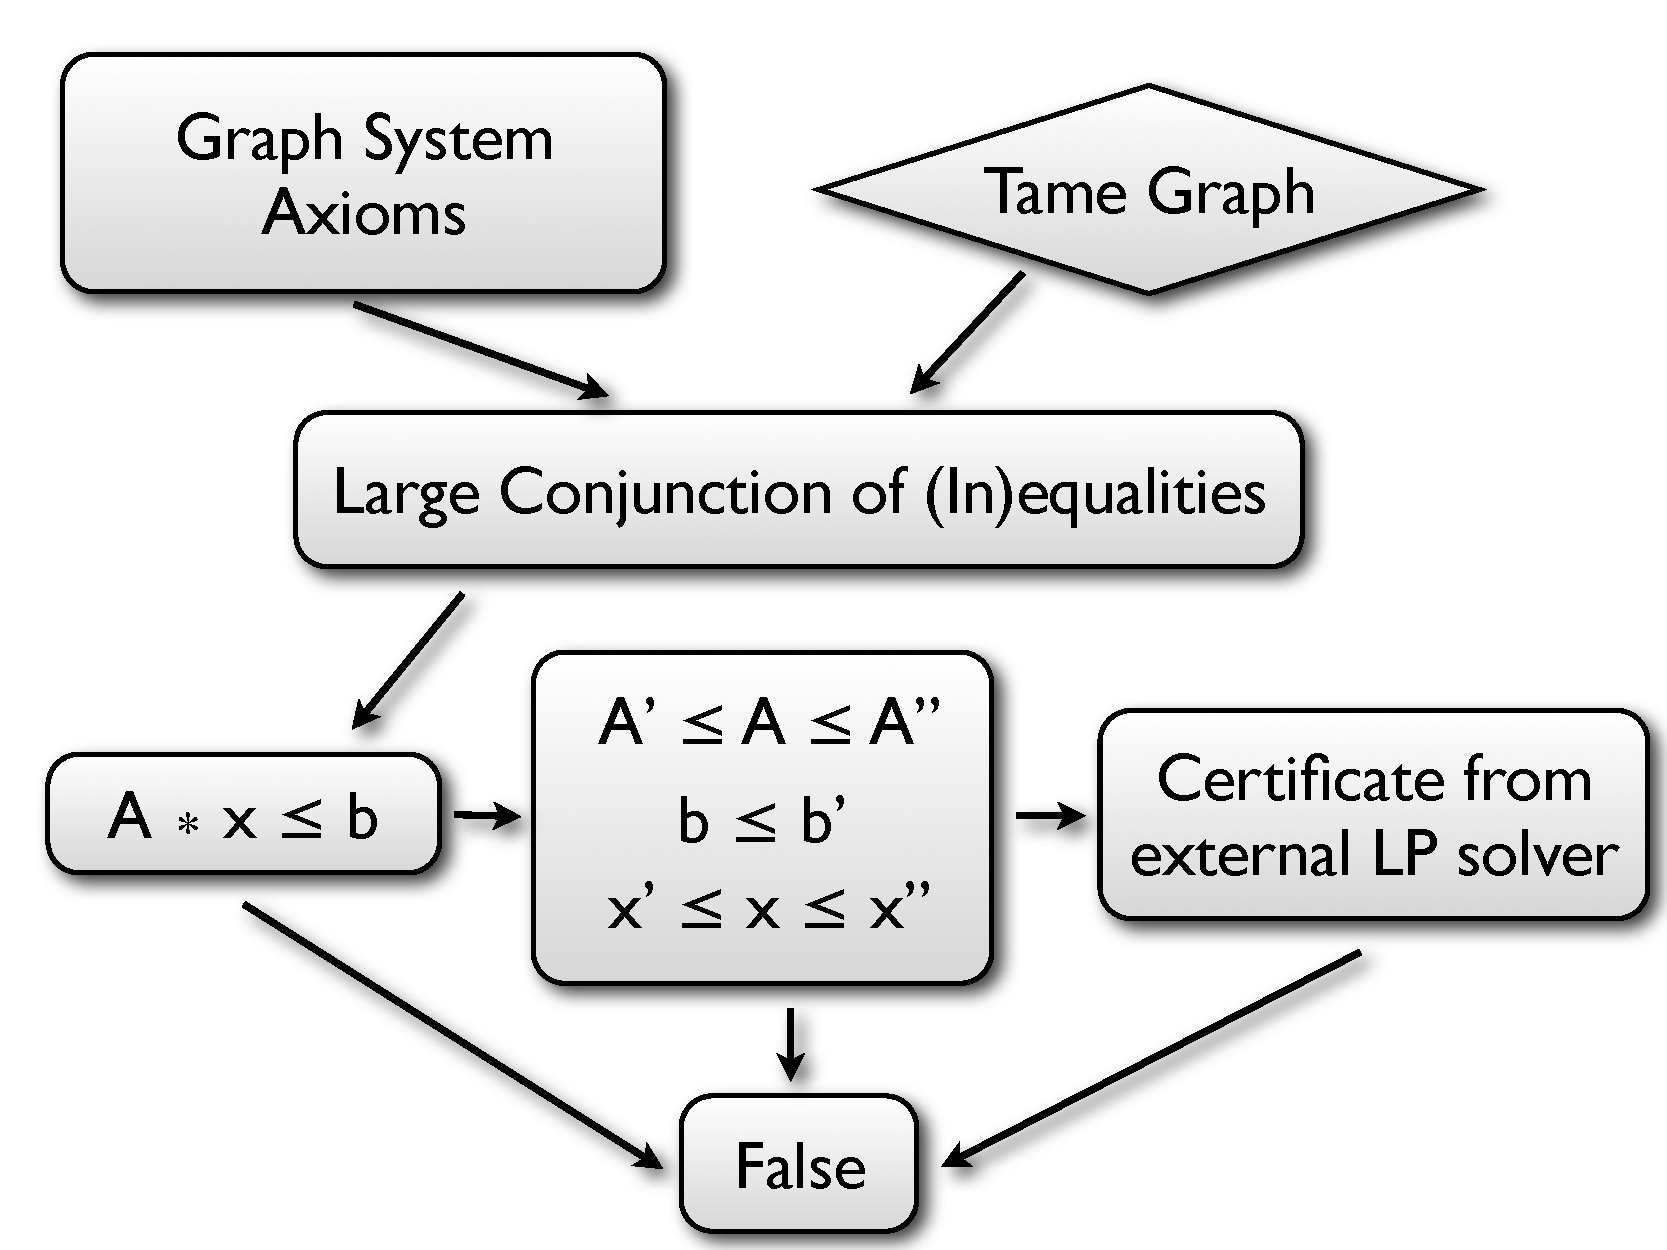
\includegraphics[width=10cm]{lpapproach}
\end{center}
\caption{Refuting a potential counterexample to the Kepler Conjecture}
\label{fig:lpapproach}
\end{figure}


\section{Biconnected graphs}


This section gives further detail to the argument of \cite[Sec.12.7~p.131]{Hales:2006:DCG}.  There it is claimed that
the proof of the main estimate \cite[Theorem~12.1]{Hales:2006:DCG} can be reduced to polygonal standard regions.
This claim is correct. 
However, the justification of this claim is not complete in the original proof. 

What Section~12.7 fails to consider
is a hypothetical situation such as that shown in Fig.~\ref{fig:biconnected}, where the rigid movement of set of vertices (such as the illustrated triangle with vertex $w$)
is blocked by a nearby vertex $v$ that is not visible at $w$, when the distance between $v$ and $w$ drops
to the minimum value $2$.  This section sketches a proof that this hypothetical situation does
not occur.\footnote{This issue only comes up in the proof of the Kepler conjecture, and not
in the proof of the dodecahedral conjecture~\cite{Hales:2008:Dodec}.  In the proof of the dodecahedral conjecture there are no loops of anchored simplices, and without loops there are no difficulties: edges of length at most
$\sqrt8$ can be be used instead of the set $E'$ below.  Lemmas~\ref{lemma:prelim},~\ref{lemma:291} are all that is needed.}  



\begin{figure}
\begin{center}
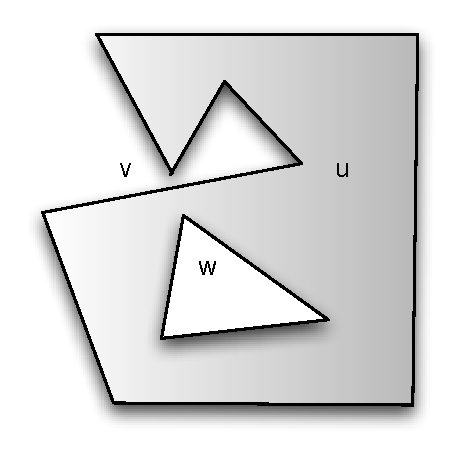
\includegraphics[width=5cm]{biconnected}
\end{center}
\caption{In this figure (not to scale), segments represent geodesic arcs on the unit sphere.  The shaded region is a subregion whose boundary is not a simple polygon.
We wish to rigidly rotate the triangle containing the vertex $w$ until a new visible distinguished edge forms
(say from $w$ to $u$).  We will show that this rigid motion does not decrease the distance between
two vertices (say $w$ and $v$)  to the minimum distance $2$.}
\label{fig:biconnected}
\end{figure}


\subsection*{Context}

We work in the following context.  We adopt notation, definitions, and conventions without further comment
from \cite{Hales:2006:DCG}.  We recall some further context.
As described in Section~12.6 of that article, we assume that all upright quarters
are erased, except loops (that is those surrounded by anchored simplices).  We fix a packing centered at a vertex at the origin.  Let $R$ be an exceptional standard region, and
$U$ the set of vertices of of height at most $2.51$.  As usual, we say two edges $\{u_1,u_2\}$ and $\{u_1',u_2'\}$ {\it cross}
if the interiors of the triangles formed by $\{0,u_1,u_2\}$ and $\{0,u_1',u_2'\}$ intersect.

We form the set of edges $E'$ between vertices in $U$, consisting of
\begin{itemize}
\item all standard edges; that is, $\{v,w\}\subset U$ such that $\|v-w\|\le 2.51$.
\item all edges $\{v,w\}\subset U$ of an anchored simplex, whenever the upright diagonal of the anchored simplex is an unerased loop.
\item all edges $\{v,w\}\subset U$ such that $\|v-w\|\le\sqrt8$, where $\{v,w\}$ does not cross any other edge in previous two items.  (If two of these edges cross, pick only one of them. This can only happen with conflicting diagonals
of a quad cluster.)
\end{itemize}
These edges do not cross.  A special simplex $\{0,u,v,w\}$ has one edge $\{v,w\}$ of length at least $\sqrt8$,
called the special edge.  The other vertex $u$ is called a special vertex (or corner).
Let $E=E'\setminus S$, where $S$ is the set of special edges (that
is, the edges of special simplices shared with an anchored simplex).
The edges of $S$ have lengths between $\sqrt8$ and $3.2$.
 The projection of the line segments formed by $E$ to the
unit sphere is a planar graph.
The complement of this graph in the unit sphere
is a disjoint union of connected componenents.  The closures of these connected components are called subregions.

We call a loop subregion one that contains an unerased loop.
If $R$ is a subregion that comes from a loop, then there are no enclosed vertices of height $\le 2.51$ over the
subregion.  The corners of $R$ are the anchors of the upright diagonal together with the special vertices
of the subregion.  The subregion $R$ is star convex with center point determined by the upright diagonal.
It follows that the boundary of $R$ is a simple polygon.

The graph $\Gamma$ with vertices $U$ and edges $E$ is not necessarily connected.  The aim is to deform
$U$ to create a biconnected graph (without changing the value of $\op{vor}_{0,R}(D),\tau_{0,R}(D)$).  Once the graph $\Gamma$
is biconnected, the subregions are simple polygons as desired.

The deformation of $U$ is required to satisfy the following conditions.
\begin{itemize}
\item If the graph $\Gamma$ is not connected,
the deformation acts by a rotation about the origin 
on the vertices of a single chosen connected component of $\Gamma$,
leaving all other vertices of $U$ fixed.  (For example, in Figure~\ref{fig:biconnected}, the entire triangle with vertex $w$ may be rotated.)
\item If the graph $\Gamma$ is connected, but not biconnected, with a chosen articulation vertex $a$, then
the deformation acts by a rotation about the axis $\{0,a\}$ on the vertices of a single component of $\Gamma\setminus\{a\}$,
leaving all other vertices of $U$ fixed.
\item The distance between $v,w$ remains at least $2$, for all $v,w\in U$.
\end{itemize}

The deformation stops when either of the following halting conditions are met:
\begin{enumerate}
\item $\|v-w\|\le\sqrt8$, where the edge $\{v,w\}\not\in E'$ does not cross any edge in $E'$, or
\item $\|v-w\|$ decreases to $2$ for some $v,w\in U$, and $\{v,w\}$ crosses an edge in $E'$.
\end{enumerate}

\begin{thm}\label{thm:biconnected}  
If $\Gamma$ is not biconnected, then a nontrivial deformation exists in this context. 
The second halting condition never occurs.  The deformation can always be continued until the first halting
condition holds.
\end{thm}

When $U$ is deformed until the first halting condition holds, a new edge $\{v,w\}$ can be added to $E$.
The theorem is repeated to add further edges, until a biconnected graph is obtained.  
The remainder of this section explains why the second halting condition never occurs.  For
this, we assume on the contrary, that $\|v-w\|=2$, where $\{v,w\}$ belong to different connected components
of $\Gamma$ (if $\Gamma$ is not connected) and different connected components of $\Gamma\setminus\{a\}$ (if $a$
is an articulation vertex of a connected graph $\Gamma$).  In short, we say that $v,w$ belong to
different bicomponents.  We may also, assume that $\{v,w\}$ crosses some edge of $E'$.

\subsection*{Preliminary lemmas}

\begin{lemma}\label{lemma:prelim}  Let $S=\{v,w,u_1,u_2,v_0\}$ be a set of five distinct points in $\ring{R}^3$ whose
pairwise distances are at least $2$. Suppose that the segment $\{v,w\}$ passes through
$\{v_0,u_1,u_2\}$. Assume
$$
\begin{array}{lll}
\|u_1-u_2\|\le 3.2\\
\|v_0-u\|\le 2.51,\text{ for } u \in S\\
\end{array}
$$
Then $\|v-w\|>2$.
\end{lemma}

\begin{lemma}\label{lemma:291}  Let $S=\{v,w,u_1,u_2,v_0\}$ be a set of five distinct points in $\ring{R}^3$ whose
pairwise distances are at least $2$. Suppose that the segment $\{u_1,u_2\}$ passes through
$\{v_0,v,w\}$. Assume
$$
\begin{array}{lll}
\|u_1-u_2\|\le 2.91\\
\|v_0-u\|\le 2.51,\text{ for } u \in S\\
\end{array}
$$
Then $\|v-w\|>2$.
\end{lemma}



\begin{proof} Both lemmas follow by geometric considerations.
\end{proof}

By these two lemmas, we may assume that for each edge $\{u_1,u_2\}$ that $\{v,w\}$ crosses,
we have that $\{u_1,u_2\}$ passes through $\{0,v,w\}$ and that $\|u_1-u_2\|>2.91$.  This means that the edge $\{u_1,u_2\}$ is an edge of an anchored simplex,
so that the edge is special or bounds a loop subregion.
This loop subregion will provide the key to the proof, because we will show
that it prevents the distance between $v$ and $w$ from becoming $2$,
as assumed  (Fig.~\ref{fig:biconnectedloop}).

\begin{figure}
\begin{center}
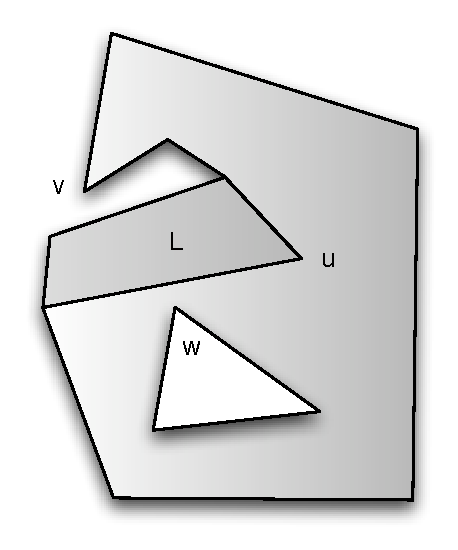
\includegraphics[width=5cm]{biconnectedloop}
\end{center}
\caption{The situation of Fig~\ref{fig:biconnected} does not exist
(as will be shown).  There is an intervening loop subregion $L$ (not to scale) that forces
$v$ and $w$ to be more than the minimum distance apart.}
\label{fig:biconnectedloop}
\end{figure}


\subsection*{Multiple edge crossings}

We break the proof of Theorem~\ref{thm:biconnected} into cases according
to the number and combinatorial structure of the edges $\{u_1,u_2\}$
that pass through the triangle $\{0,v,w\}$.

\begin{figure}
\begin{center}
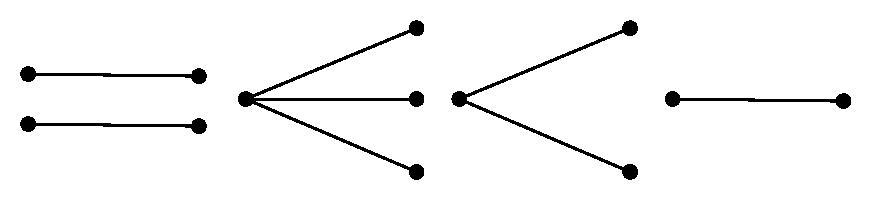
\includegraphics[width=10cm]{cases}
\end{center}
\caption{Theorem~\ref{thm:biconnected} is proved in various cases: two edges with
distinct endpoints, three or more edges, two edges, or a single edge
passing through the triangle $\{0,v,w\}$.}
\label{fig:cases}
\end{figure}

The following lemma shows that we cannot have two such edges $\{u_1,u_2\}$ and $\{u_1',u_2'\}$ with distinct endpoints.  From the lemma it follows that there is an endpoint $u_2$ shared by every edge that passes through the
triangle $\{0,v,w\}$.  Lemma~\ref{lemma:three-edge} shows that there cannot be three or more edges.  Finally, the cases of one or two edges $\{u_1,u_2\}$ are treated in further subsections (Fig.~\ref{fig:cases}).

\begin{lemma}\label{lemma:double-edge} 
There does not exist a set $S=\{0,v,w,u_1,u_2,u_1',u_2'\}$ of seven distinct points
in $\ring{R}^3$ whose pairwise distances are at least $2$ and that satisfies the following conditions.
\begin{itemize}
\item The edges $\{u_1,u_2\}$ and $\{u_1',u_2'\}$ do not cross.
\item The edges $\{u_1,u_2\}$ and $\{u_1',u_2'\}$ both pass through $\{0,v,w\}$.
\item $\|u\|\le 2.51$ for all $u\in S$.
\item $\|v-w\|=2$.
\item $\|u_1-u_2\|,\|u_1'-u_2'\|\le 3.2$.
\end{itemize}
\end{lemma}

\begin{proof}
Assume $S$ exists.  We may label vertices so that $u_1$ and $u_1'$ lie in the same half-space bounded by
the plane through $\{0,v,w\}$.   We may label so that the directed
segment from $v$ to $w$ crosses the edge $\{u_1',u_2'\}$
before the edge $\{u_1,u_2\}$.

We claim that $\|v-u_2\|$ or $\|w-u_2\| > 2.7$.  For a contradiction, assume that both
are at most $2.7$.  By geometric considerations, $u_2'$ is not enclosed over $\{v,w,u_2\}$.
This implies that $(w_1,w_2,w_3,w_4)=(u_2',u_2,w,u_1')$ occur in cyclic order around $\{0,v\}$.
Set $d(i,j) = \op{dih}(0,v,w_i,w_j)$.  Then $d(0,4)\le \pi$.
We make pivots that preserve the constraints, maintain $d(0,4)\le \pi$, and contract $\|u_1'-u_2'\|$.
By considering the value of $\Delta$, we find that if any of the following conditions hold, then $\{0,v,u_1',u_2'\}$ cannot be collinear, and the condition
$d(0,4)<\pi$ forcibly holds: $\|v\|\le 2.39$, $\|u_1'\|\ge 2.15$, $\|u_2'\|\ge 2.15$, $\|v-u_1'\|\ge 2.15$, $\|v-u_2'\|\ge 2.15$.
Furthermore, when $d(0,4)<\pi$, pivots can be used to deform the configuration until
$\|v\|\ge 2.39$, $\|u_1'\|\le 2.15$, $\|u_2'\|\le 2.15$, $\|v-u_1'\|\le 2.15$, and $\|v-u_2'\|\le 2.15$.  Thus, 
we may assume these conditions.  Now disregard the constraint $\|u_1'-u_2'\|\le 3.2$.  Continue with deformations
that decrease $d(0,4)$ and move $u_2,w$ until $\|u_2'-u_2\|=2$, $\|u_2-w\|=2$, $\|w-u_1'\|=2$, $\|v-u_2\|=2.7$, $\|v-w\|=2$, $\|u_2\|=2.51$, $\|w\|=2.51$.
An interval calculation\footnote{8167927350} now gives the contradiction
  $$d(0,4) = \sum_{i=0}^2d(i,i+1) > \pi.$$
%Suppose first that $u_2'$ is enclosed over $(0,\{v,w,u_2\})$. 
%
%Now $u_2'$ is not enclosed over $(0,\{v,w,u_2\})$.  As $\{v,w\}$ crosses, $\{u_1',u_2'\}$, we must
%have that $\{u_1',u_2'\}$ crosses $\{v,u_2\}$.  We claim that $\|v-u_2\|\ge 2.7$.  For otherwise,
%if $\|v-u_2\|\le 2.7$, we can use geometric considerations to contract $\{u_1',u_2'\}$ until
%$$
%\begin{array}{lll}
%\|u_1'-w\|=2,&\|w-u_2\|=2,&\|u_2-u_2'\|=2,\\
%\|w\|=2.51,&\|v-u_2\|=2.7,&\|u_2\|=2.51.
%\end{array}
%$$
%A calculation of the dihedral angle gives a contradiction:
%$$
%\begin{array}{lll}
%\pi &\ge\op{dih}(0,v,u_1',u_2') = \op{dih}(0,v,u_1',w)+\op{dih}(0,v,w,u_2)+\op{dih}(0,v,u_2,u_2')\\
%&=\dih(y,y_2,2,2,2,y_3)+\dih(y,2.51,2.51,2,2,2.7)+\dih(y,y_4,2.51,2,2.7,y_5) \\
%  &>\pi.
%\end{array}
%$$
%We take $\|v-u_2\|\ge 2.7$.  Symmetrical arguments give $\|v-u_1\|\ge 2.7$, $\|w-u_1'\|,\|v-u_2'\|\ge 2.7$.
%The edge $\{u_1,u_2\}$ passes through $\{0,v,w\}$.  Geometrical considerations show that $\|u_1-u_2\|>3.2$
%unless $\|u_2\|\le 2.16$, $\|u_2-w\|\le 2.17$, $\|w\|\ge 2.36$.  Corresponding estimates  hold with
%$u_2$ and $u_1$ interchanged.  Then a calculation\footnote{BB} gives a contradiction
%$$
%\pi \ge \op{dih}(0,w,u_1,u_2) = \op{dih}(0,w,u_1,v) + \op{dih}(0,w,v,u_2) >
%2 (\pi/2).
%$$

By symmetry, we have $\|v-u_1\|$ or $\|w-u_1\|>2.7$.  By symmetry, we reduce to two cases.

{\it Case 1:}  $\|v-u_2\|>2.7$ and $\|w-u_1\|> 2.7$.  In this case, geometric considerations
give the contradiction:  $\|u_1-u_2\| > 3.2$.

{\it Case 2:}  $\|w-u_1\|>2.7$ and $\|w-u_2\|>2.7$.  Geometric considerations lead to the contradiction
$|u_1-u_2|>3.2$, unless $\|w\|\le 2.36$, $\|u_2\|\le 2.16$, $\|w-u_2\|\le 2.17$.  An interval calculation\footnote{6040218010}
shows that
$\op{dih}(0,w,v,u_2)>\pi/2$.
Similarly, $\op{dih}(0,w,v,u_1)>\pi/2$.  We reach the contradiction
$$
\pi > \op{dih}(0,w,u_1,u_2) > \pi/2 + \pi/2.
$$
\end{proof}

By this lemma, there is a common endpoint $u_2$ such that every edge
of $E'$ that passes through $\{0,v,w\}$ has $u_2$ as an endpoint.
Next we show that there cannot be three such edges.  


\begin{lemma}\label{lemma:three-edge}
There does not exist a set of seven distinct points
$$S=\{0,v,w,u_1,u_1',u_1'',u_2\}$$ in $\ring{R}^3$ that satisfies
the following conditions.
\begin{itemize}
\item The distance between each pair of distinct points in $S$ is at least $2$.
\item The edges $\{u_1,u_2\}$, $\{u_1',u_2\}$, and $\{u_1'',u_2\}$ pass through
$\{0,v,w\}$.
\item $\|u\|\le 2.51$, for all $u\in S$.
\item $\|v-w\|=2$.
\item $\|u-u_2\|\le 3.2$, for $u=u_1,u_1',u_1''$.
\end{itemize}
\end{lemma}

\begin{proof}
We may order the vertices in cyclic order around $\{0,u\}$ as
$$(w_1,w_2,w_3,w_4,w_5)=(w,u_1,u_1',u_1'',v),$$ 
so that setting
$d(w_i,w_j) = \dih(0,u_2,w_i,w_j)$, we have
$$d(w_1,w_5)=\sum_{i=1}^4 d(w_i,w_{i+1})\ge d(w_2,w_3)+d(w_3,w_4).$$
Interval calculations\footnote{2799256461, 5470795818} 
give $d(w_2,w_3),d(w_3,w_4)\ge 0.7$
and $d(w_1,w_5)< 1.4$. We obtain an immediate contradiction:
$$1.4 > d(w_1,w_5) \ge 0.7 + 0.7.$$
\end{proof}

\subsection*{Double edge crossings}

This subsection treats the case of two edges crossings in the proof
of Theorem~\ref{thm:biconnected}.
In this subsection, we continue to assume the general context of Theorem~\ref{thm:biconnected}.  As usual, 
the edge $\{u_1,u_2\}\in E'$ crosses $\{v,w\}$.

\begin{lemma}\label{lemma:special}
Let $\{u_1,u_2,w,v\}$ be a set of four distinct points
in $\ring{R}^3$ (in the given context).  
Assume that
 $\|v-u_i\|\le 2.51$, for $i=1,2$.
Assume that no edge of $E'$ crosses $\{v,w\}$
in the open 
half-space $A$ containing $v$ bounded by the plane $\{0,u_1,u_2\}$.
(That is, $\{u_1,u_2\}$ is the first edge to cross $\{v,w\}$, moving
from $v$ toward $w$.)
Assume there is a loop subregion $L$ along 
$\{u_1,u_2\}$ on the $A$-side
of $\{u_1,u_2\}$.  Then $\{u_1,u_2\}$ is a special edge of $E'$ with
corner $v$.
In particular, $\{u_1,u_2\}\not\in E$, so that it is not a bounding
edge of a subregion.
\end{lemma}

\begin{proof}
Assume for a contradiction that $\{u_1,u_2\}$ is not special.
Note that loop subregions have simple polygonal boundaries and
remain rigid under all the deformations.  In particular,
the upright diagonal, special corners, and so forth
remain rigidly positioned with respect to the corners of the subregion.

Since there are no further edges crossing $\{v,w\}$, the subregion
$L$ extends to $v$.  Hence $v$ is a corner of the subregion $L$.
It is either an anchor or a special corner (with respect to $L$). However, it cannot be a special
corner, by the assumption that $\{u_1,u_2\}$ is not a special edge.
Hence it is an anchor.  Also, $u_1$ and $u_2$ are anchors.

To reach a contradiction, 
we consider possible locations of the upright diagonal $\{0,u\}$,
and show that it has nowhere to go (Figure~\ref{fig:nogo}).  
Since $u_1,u_2$ form an edge,
they are consecutive anchors (excluding region $B$).  
Also, the upright diagonal of any
unerased loop has at least four anchors.  Geometric considerations show that
the fourth anchor is not in $A$.  This prevents $u$ from
being located over the region $A$.
A vertex $u_2$ cannot be enclosed over an upright quarter $\{0,u,v,u_i\}$.  This excludes
 region $C$.  Finally, an edge $\{v,u_i\}$
of length at most $2.51$ cannot pass through a triangle $\{0,u,u_j\}$
of sidges at most $2.51,2.51,\sqrt8$ (excluding $D$).
\end{proof}

\begin{figure}
\begin{center}
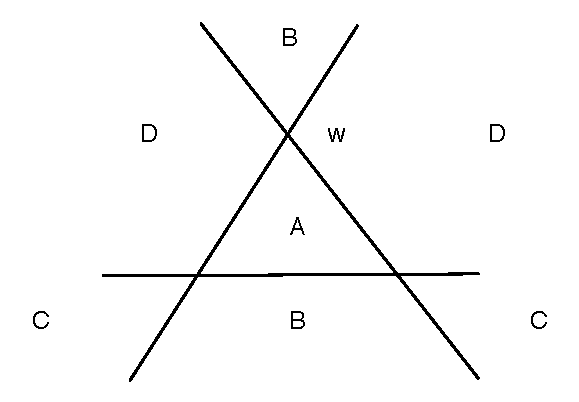
\includegraphics[width=5cm]{nogo}
\end{center}
\caption{The upright diagonal $u$ cannot be placed over any of
the regions $A,B,C,D$.  The lines (not to scale) represent geodesic arcs on the
sphere passing through the pairs of points in $\{p(u_1),p(u_2),p(w)\}$,
where $p$ denotes projection to the unit sphere.}
\label{fig:nogo}
\end{figure}

\begin{lemma}\label{lemma:circuit} 
Let $\{u_1,u_2,w,v\}$ be a set of four distinct points
in $\ring{R}^3$ (in the given context).  
Assume that
 $\|v-u_i\|\le 2.51$, for $i=1,2$.
Assume that no edge of $E$ crosses $\{v,w\}$
in the open 
half-space $A$ containing $v$ bounded by the plane $\{0,u_1,u_2\}$.
(That is, $\{u_1,u_2\}$ is the first edge to cross $\{v,w\}$, moving
from $v$ toward $w$.)
Then 
both edges $\{u_1,v\}$ and $\{u_2,v\}$ belong to $E$.
In particular, there is a circuit of the graph $\Gamma$ through $v,u_1,u_2$.
\end{lemma}

\begin{proof} Under the assumption that 
there is a loop subregion $L$ along 
$\{u_1,u_2\}$ on the $A$-side
of $\{u_1,u_2\}$, Lemma~\ref{lemma:special} implies that
$\{u_1,u_2\}$ is a special edge of $E'$ with
corner $w$.  In particular, $\{u_1,v\}$ and $\{u_2,v\}$ are
edges of $E$.  Now assume that there is no loop subregion along
$\{u_1,u_2\}$ on the $A$ side of $\{u_1,u_2\}$.

Let $S$ be the finite set of points of $U$ enclosed
over the simplex $\{0,u_1,u_2,v\}$.  We show by contradiction
that $S$ is empty.
The plane $\{0,v,w\}$ separates
$S$ into a disjoint union $S = S_1\cup S_2$, according to those
in the same half-space as $u_i$, $i=1,2$.
We form the convex hull of the projection $p$ to the unit sphere of the 
points $S_i\cup\{u_i,v\}$.  As in~\cite[Sec.~12.13]{Hales:2006:DCG},
form a sequence of geodesic arcs on the unit sphere from $p(u_i)$
to $p(v)$.  Let $p(w_i)$, for $w_i\in S_i$, be the other endpoint
of the arc starting at $p(u_i)$.  Either $p(w_1)$ is contained in the
triangle $\{p(u_1),p(u_2),p(w_2)\}$, or
$p(w_2)$ lies in the triangle $\{p(u_1),p(u_2),p(w_1)\}$.  Assume
the former.  Then the edges $\{w_1,u_i\}$ do not cross any edges
of $E$.  Furthermore, geometric considerations show that
$\|w_1-u_i\|\le 2.51$, for $i=1,2$.  By the criteria for forming
edges of $E$, we must have $\{w_1,u_i\}\in E$ for $i=1,2$.  This
contradicts the assumption that $\{v,w\}$ does not cross any edges
of $E$ over $A$.  Hence $S=\emptyset$.

Since $S=\emptyset$, the edges $\{v,u_i\}$ do not cross any edges
of $E$.  By the criteria for forming edges of $E$, they belong to $E$.
This completes the proof.
\end{proof}

We are ready to prove the next major case of Theorem~\ref{thm:biconnected}.
We continue to work in the general context of that theorem, with $v$ and $w$
in different bicomponents of the graph $\Gamma$.

\begin{lemma}\label{lemma:double-cross}  
In this context, there does not exist six points $\{0,v,w,u_1,u_1',u_2\}$
where $\{u_1,u_2\}$ and $\{u_1',u_2\}$ pass through $\{0,v,w\}$ and such that
  $$\|u_1-u_2\|\le 3.2,\quad \|u_1'-u_2\|\le 3.2.$$
\end{lemma}

\begin{proof}  By the previous results, there are at most two edges that pass through $\{0,v,w\}$
in this manner.  In particular, the part of the line segment $\{v,w\}$ between the crossings
of $\{u_1,u_2\}$ and $\{u_1',u_2\}$ lies in a single loop subregion.  It follows from this that
$\{u_1,u_2,u_1'\}$ are corners of the same loop subregion.  Hence, they lie on a circuit in $\Gamma$
formed by the corners of that loop subregion.  

We may assume that $\{u_1,u_1'\}$ are ordered so that the cyclic order around $\{0,u_2\}$ is
$(w_1,w_2,w_3,w_4)=(v,u_1',u_1,w)$.  If $\|v-u_2\|,\|v-u_1'\|\le 2.51$, then by Lemma~\ref{lemma:circuit}, the points
$\{v,u_1',u_2\}$ lie on a circuit in $\Gamma$.  A similar conclusion holds if corresponding inequalities
hold $\|w-u_2\|,\|w-u_1\|\le 2.51$.  If all four inequalities hold, then these circuits put $v,w$ in the
same bicomponent of $\Gamma$, which is contrary to hypothesis.  Hence we may assume by symmetry and without
loss of generality that $\|v-u_1'\|\ge 2.51$ or $\|v-u_2\|\ge 2.51$.  
We may stretch along the edges $\{u_2,u_1\}$, $\{u_2,u_1'\}$, moving $u_1,u_1'$, 
until $\|u_2-u_1\|=\|u_2-u_1'\|=3.2$.   We may add inequality
$$
\|u_2\|\le 2.23,
$$
for otherwise by geometric considerations $\|u_2-u_1'\|> 3.2$.  Similarly, $\|u_1'\|\le 2.23$.
We may scale $v$ until $\|v\|=2.51$.
If $\|u_2-v\|\ge 2.51$, we may pivot $v$ toward $u_2$ around the axis $\{0,w\}$ until $\|u_2-v\|=2.51$.
Similarly, we may assume that $\|u_2-w\|\le 2.51$.
% Note that while $\|u2-w| ge 2.51$, we cannot have Delta=0, so deformations are fine.
Set $d(i,j) = \op{dih}(0,u_2,w_i,w_j)$.
Then interval arithmetic calculations\footnote{7431506800, 5568465464, 4741571261, 6915275259 } give the contradiction:
$$
1.3 > d(1,4) = d(1,2) +d(2,3)+d (3,4) > 0.5 + 0.8 + 0 = 1.3.
$$
\end{proof}

\subsection*{Single edge crossings}

This subsection treats the proof of Theorem~\ref{thm:biconnected}
in the case of a single edge crossing $\{u_1,u_2\}$.  This is
the final case of the proof.
We continue to assume the notation and general context of that theorem.
In particular, either $v$ and $w$ lie in different bicomponents of
the graph $\Gamma$.

\begin{lemma}  Let $\{0,u_1,u_2,v,w\}$ be a set of five distinct
points such that $\{u_1,u_2\}$ is the only edge of $E'$ that
crosses $\{v,w\}$.  Then $\|v-w\|>2$.
\end{lemma}

\begin{proof} We assume for a contradiction that $\|v-w\|=2$.
We consider four cases depending on lengths.  

{\it Case 1:} $\|u-u_i\|\le 2.51$, for $i=1,2$ and $u=v,w$.
By Lemma~\ref{lemma:circuit}, there are circuits running through
$\{u,u_1,u_2\}$, for $u=v,w$.  This is contrary to the assumption
that $v,w$ lie in different bicomponents of the graph $\Gamma$.  (In the remaining cases, there is
no loss in generality to assume $\|w-u_2\|\ge 2.51$.)

{\it Case 2:} $\|w-u_2\|\ge 2.51$, $\|v-u_1\|\ge 2.51$.
Geometric considerations give the contradiction
$\|u_1-u_2\|>3.2$.

{\it Case 3:} $\|w-u_2\|\ge 2.51$, $\|v-u_2\|\ge 2.51$.
Geometric considerations gives the contradiction
$\|u_1-u_2\|>3.2$.

{\it Case 4:} $\|w-u_2\|\ge 2.51$, $\|v-u_i\|\le 2.51$, for $i=1,2$.
The edge $\{u_1,u_2\}$ cannot be a special edge of $E'$.  Otherwise,
$v,w$ are corners of the same loop subregion.  This contradicts
the running assumption that these two vertices belong to separate
bicomponents of the graph $\Gamma$.  By Lemma~\ref{lemma:special}, there is no loop subregion along $\{u_1,u_2\}$ on the $v$-side.
Since $\{u_1,u_2\}$ has length greater than $\sqrt8$, there
is a loop subregion $L$ bounded by the edge, and it must then lie
on the $w$-side.  Thus, $w$ is a corner of $L$ and the circuit of
$\Gamma$ described by the boundary of $L$ passes through $w,u_1,u_2$.
By Lemma~\ref{lemma:circuit}, there is a circuit of $\Gamma$ through
$v,u_1,u_2$.  Hence, $v,w$ lie in the same biconnected component,
which is contrary to the running assumption.
\end{proof}



%\twocolumn
\section{Errata}


The abridged version of the Kepler conjecture
in the Annals \cite{Hales:2005:Annals}
was generated by the same tex
files as the unabridged version in \cite{Hales:2006:DCG}.
For this reason,
it seems that every correction to
the abridged version should also be a correction to the unabridged version.
We list the errata for the
unabridged version. The same list applies to corresponding 
passages in the abridged version.  



Each correction gives its location in \cite{Hales:2006:DCG}.
The location
\line+n counts down from the top of the page, or
if a section or lemma number is provided, it
counts from the top of that organizational unit.
The location \line-n counts up from the bottom
of the page. Footnotes are not included in the
count from the bottom.  Every line containing
text of any sort is included in the count,
including displayed equations, section headings,
and so forth.  The material to the left of $\lto$ 
indicates original text, and material to the right of the
arrow gives replacement text.  
The original text and replacement text appear in italic.
Comments about the corrections appear in roman. 
Please report further errors to Hales.


In addition to the corrections to the text mentioned below, 
there have been some corrections to the computer code, including some typos in the
listings of nonlinear inequalities.
They are described in detail in~\cite{Hales:2008:Errata}.


\subsection*{Listing}\hfill\break
\parskip=0.2\baselineskip

\begin{\sz}
\baselineskip=1.2\baselineskip

[p.47,Lemma~5.16] $Q\lto F$

[p.49,\line+2] {\it supposed} \lto {\it suppose}
	
[p.63,Lemma~7.10]
	${\mathcal S}$-{\it system} \lto $Q$-{\it system}
	
[p.73][p.124] {\rmx Some applications (such as Lemma~11.24) of Theorem~8.4 rely on
the proof of the theorem, which is more general than
the statement of the theorem.  There are no errors or gaps here,
but the wording of the theorem should have been phrased differently
so that it would not have been necessary to refer to the proof.  The proof is based on a finer
decomposition into pieces.  These finer pieces are sometimes used.}

[p.75,Remark~8.11]
	{\it show}\lto {\it shows}

[p.78,\line-7] {\it constraints} \lto{\it  constraint}

[p.86,\line+14] {\it Let $\{0,v\}$ be 
          the diagonal of an upright quarter in the $Q$-system
        \lto
       Let $v$ be a vertex with $2t_0<|v|<\sqrt8$.}
           {\rmx Section~9 assumes that the diagonal belongs to
          a quarter in the $Q$-system, but Lemma~10.14 uses these
          results when $\{0,v\}$ has $0$ or $1$ anchors.  To make
          this coherent, we should assume throughout Section~9 that
          we have the weaker condition that whenever $\{0,v\}$ has
          two or more anchors it is a diagonal of a quarter in the $Q$-system.
          The proofs of Section~9 all go through in this context.
           (Lemma~9.7 is all that is relevant here.)}

[p.87,Definition~9.3]
	{\rmx In definition of $\Delta(v,W^e)$, we
	can have some $Q$ (as in Fig~9.1)
	with negative orientation.
	In this case, $E_v\cap E_i$ can clip
	the other side.  We want the object
	without clipping.   $\Delta(v,W^e)$ should be understood as the
        unclipped object.}
	
[p.88,Definition~9.6]
	{\rmx The definition is poorly worded.  First of
	all, it requires that the subscript to
	$\epsilon$ should be a vertex, but then in
	the displayed equation, it makes $w/2$ the
	subscript, which is not a vertex.   To
	define $\epsilon'$, move from $w/2$ along
	the ray through $x'$ until an edge of the
	Voronoi cell is encountered.  If $v,w,u$
	are the three vertices defining that edge,
	then set $\epsilon'_v(\Lambda,x)=u$.
	Degenerate cases, such as when two different
	edges are encountered at the same time,
	can be resolved in any consistent fashion.  In~\cite{hales:2008:collection},
      these degeneracies are avoided altogether, by replacing functions 
      $\epsilon,\epsilon'$ with sets $\Phi,\Phi'$.
     }
	
[p.88,Lemma~9.7,\line+2] 
	$w$\text{{\it  and} } $v$\lto $w$ \text{ {\it and} } $u$

	
[p.88,L.~9.7,Claim~1]
	\text{{\it  with }} $|w - w'|\le 2t_0$, \text{ {\it and} }
	\lto \text{ {\it with} }

	
[p.88,L.~9.7,\line+5]
         {\it Then: $\lto$ Let
          $
          R'_w = \{x\in R_w \cap(0,\{u,w\})\mid 
          \epsilon_0(x,\{u,w\}) = u.
          $
          Assume that $R'_w$ is not empty. Then:}
         %{\rmx (This hypothesis is satisfied
        %in every application of Lemma~9.7.
        %We note that this forces the orientation of $\{0,v,w'\}$ to
        %be negative in $Q=\{0,v,w',u\}$, which in turn forces $Q$
        %to be a quarter.)}

[p88,L.~9.7,Claim~3]
        $R_w \lto R'_w$

[p.89,\line+2]
	$
	\{w,v\}\lto\{w,u\}
	$

[p.92,\line+16,\line+21]
   $     \max_j u_j \lto \max_j |u_j|$
	
[p.93,\line-4]
	$
	\text{{\it obstructed from} }w \lto
	\text{{\it obstructed from} }w'
	$
		
[p.93,\line-2]
	$
	\text{{\it from some}} \lto \text{{\it for some}}
	$

[p.99,\line+1]
        $
        \text{{\it start}} \lto \text{{\it star}}
        $

[p.105,Lemma~10.14]  {\rmx In the proof of the cases involving
   $0$ or $1$ anchor, a combination of the decompositions from
   Section~8.4 and Section~9 are used.  These decompositions haven't
   been shown to be compatible.  
   Instead, it is better to combine
   $\Delta(v,W)$ with $t_0$-truncation on the rest of the quad-cluster.
   With a $t_0$ truncation, we no longer have the non-positivity results
   from Section~8.  (The quoins give a positive contribution.) However,
   I have checked that
   the estimate on $\Delta(v,W)$ is sufficiently small so that we still
   obtain a constant less than $-1.04\,\op{pt}$.}
   

[p.116][p.121] {\rmx Definition~11.7 allows masked
flat in definition of $3$-unconfined.
Definition~11.24 requires no masked flats
in the same definition.  Use Definition~11.24 (no masked flats), rather than~11.7.  
Where masked flats occur,
treat them with Lemma~11.23, parts (1) and (2).}

[p.116,\line+1] 
	$
	\text{{\it Lemma}}~4.16 \lto \text{{\it Lemma}}~4.17
	$

[p.117,before Lemma~11.9]
	$
	\text{\it two others} \lto \text{\it three others}
	$
	
[p.117,Def~11.8]
    $
    y1 \lto y_1
    $
    
 
[p.119,Definition~11.5]  {\rmx By definition, we require a masked flat quarter to
be a strict quarter.}
	
[p.121] {\rmx See p.116.}

[p.121,\line-5]
	$
	0.2274 \lto 0.02274
	$


	
[p.123. flat case (2)]  {\rmx It is missing
isolated quarters cut from the side.
To fix this, in condition 2(f), }
	$
	\eta_{456}\ge\sqrt2 \lto
	\eta_{456}\ge\sqrt2 \text{\it or } \eta_{234}\ge\sqrt2.
	$
	
[p.124] {\rmx See p.73. }
	
[p.126]  {\rmx Theorem~12.1 needs to be stated in
a form that allows the application in pp.251-252
and Lemma~13.5.  In these applications, the
regions are smaller than standard regions.
Yet in the statement of the theorem, the regions
are standard regions.  This is not a problem
in practice, because the proof is at a much
finer level of decomposition than standard regions.
However, the wording should to be changed so
that the theorem applies precisely.}


[p.126] 
{\rmx Theorem~12.1 should include $\sigma_R(D)\le s_n$
with $s_3 = 1\,\op{pt}$ and $s_4=0$, and
$\tau_R(D) \ge t_3 = 0$.}

[p.131] {\rmx There is a long note in a separate section above about
the deformation arguments on this page that produce a biconnected graph.}


[p.139,Lemma~12.18,proof,\line+3] 
	$C_0(|v|,\pi) \lto
	C_0^u(|v|,\pi)
	$
	
[p.139,Lemma~12.18] 
	$
	\tau_0(C_0^u(2t_0,\pi))-\pi_{\text{max}}\lto
	\tau_0(C_0^u(2.2,\pi))-\pi_{\text{max}}
	$

[p.144,\line+11,\line+17]
	$2t_0^2 \lto (2t_0)^2
	$

%c
[p.146]
		$S_n^\pm$ \lto
	{\it of 3-crowded, 3-undefined, and
	4-crowded combinations}

%c	
[p.148,Sect. 13.6]  {\rmx This entire
section is misplaced.  It belongs with
Sections 25.5 and 25.6.}

%c
[p.149,before 13.7]
{\it the diagrams\lto
	Figs~25.1--25.4}

%c	
[p.149,p.156] {\rmx The definition of $\delta_{loop}$ was accidently
dropped from the published version.  Set $\delta_{loop}(5,1)=0.24939$.
% Defined 1998 of kepler.tex,
}

[p.156,Lemma~13.5,\line+4]
	{\it respectively for $\tau_R(D)$\lto
	respectively, for $\sigma_R(D)$ and }
	$\tau_R(D)$ 

%c
[p.164,\line-1] 
	{\it This shows$\ldots$ occur.
	\lto This completes the proof.}


%c
[p.173,\line+4] {\rmx Insert the subscript on $b$,
as in Proposition~15.5, starting on page 173:}
   $b$ \lto $b_q$.



	
[p.182,Lemma~16.7]  {\rmx The bound of $0$ has not been
shown to hold on each half.  This is not a 
direct consequence
of Theorem~8.4. as claimed.
This can be fixed as follows.  Show by an interval arithmetic
calculation that each side separately satisfies
that bound $0$ if each vertex has height at most $2.3$ (Calculation I\_5127197465).
% HXX
If any vertex has height greater than $2.3$ show that the $\op{vor}_0$-scored quad cluster scores
less than $-1.04\,\op{pt}$.  
For this, we may use the deformations of Lemmas~12.10 and 13.1.  We may also use calculation I\_474496219, which shows that if the diagonal reaches $2\sqrt2$, each half is at most $0.009$.  
By these deformations and this calculation, the result now follows from Calculation I\_7710172071.}
% HXX


[p.241]  {\rmx `Mixed' is defined so as to include
the pure analytic case.  In earlier papers,
`mixed' excludes the pure analytic.  }
	{\it mixed\lto mixed or pure}
	
[p.243,\line+13,\line+14,\line+15]
	{\rmx Delete three sentences:}
	{\it `Let $v_{12}$ be $\ldots$  We let $\ldots$
	 Break the pentagon $\ldots$'}
	
[p.248,last displayed formula]  
	$=$ \lto $+$
{\rmx so that it reads}
	$$
	\sum_i f_{R_i}(D) \le \hat\sigma(Q_i) +
	\op{vor}_{R',0}(D) + \pi_R
	$$

[p.252,Sec.~25.7,Cases~2 and 3]  {\rmx `The flat quarter'
is mentioned, but there are no flat quarters
that have been introduced into the context.  
This passage
has been displaced from its original context.}

[p.254,\line+7]
{\it to branch combine \lto to combine}
\end{\sz}



\bibliographystyle{abbrv}
\bibliography{all}

\bigskip

\begin{\sz}
\svninfo
\end{\sz}






\end{document}
